\documentclass{report}
\usepackage[utf8]{inputenc}
\usepackage{amsmath}
\usepackage{graphicx,float}
\usepackage{caption}
\usepackage{subcaption}
\usepackage{gensymb}
\usepackage[margin=1.25in]{geometry}
\usepackage[numbered,framed]{matlab-prettifier}
\usepackage{tikz}
\usepackage{pdfcomment}
\newcommand{\matr}[1]{\mathbf{#1}} % undergraduate algebra version
\usepackage{emptypage}

\title{Optimization of an Axisymmetric, Cardioid Loudspeaker}
\author{Alex Booth, supervised by Jonathan Hargreaves\\ a.booth9@edu.salford.ac.uk}

\begin{document}
\pagenumbering{roman}
%titlepage
\begin{center}
    \thispagestyle{empty}
\begin{minipage}{0.75\linewidth}
    \centering
%University logo
    
\includegraphics[width=0.75\linewidth]{figs/Logo.jpg} \\
    \hrule
    \vspace{3cm}
%Thesis title
    {\uppercase{\Large Optimization of an Axisymmetric, Cardioid Loudspeaker\par}}
    \vspace{3cm}
%Author's 
    {\Large Alex Booth (@00513534), supervised by Dr. Jonathan Hargreaves\par}
%Degree
    {\Large A dissertation submitted for a Bachelor's of Engineering in Audio and Acoustical Engineering.\par}
    \vspace{3cm}
%Date
    {\Large May 2023}
\end{minipage}
\end{center}

\begin{abstract}
    This dissertation describes an investigation into the real-world directivity over frequency of a prototype axisymmetric, cardioid loudspeaker.
    Far-field directivity measurements of this prototype loudspeaker were taken and analyzed.

    From this analysis a metric of cardioid directivity was derived, the metric was used to construct a digital filter that would aim to encourage cardioid directivity across the low-frequency range of the prototype loudspeaker.
    Suggestions are made as to how the filtered loudspeaker may be used as an effective tool of sound field control, with particular attention paid to loudspeaker use in contemporary sound field control literature.

    The filter is shown to analytically behave as expected with some promising combined directivity performance results.
    However, the scope of these tests was ultimately time limited, and suggestions for further work and investigations are given.
    \vspace{2cm}

    \begin{figure}[H]
        \centering
        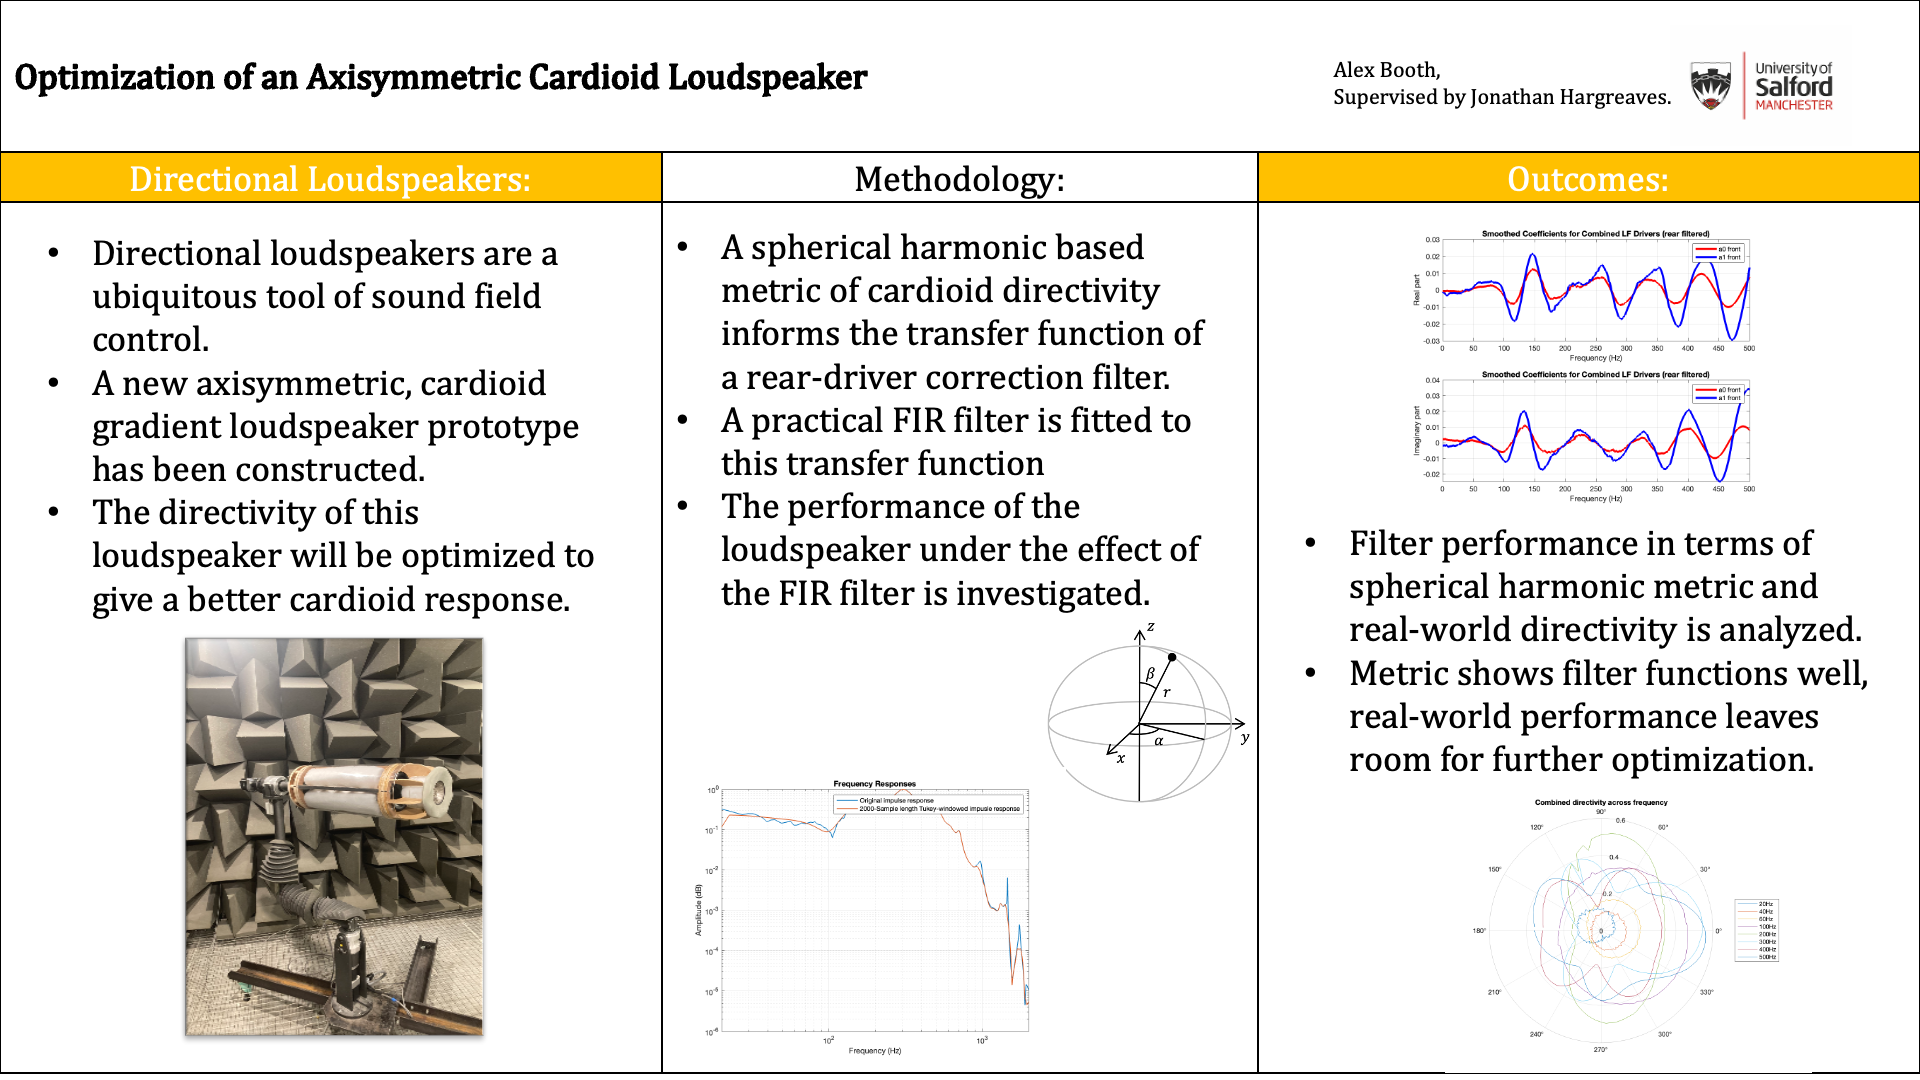
\includegraphics[scale = 0.45]{figs/visualAbstract.png}
    \end{figure}

\end{abstract}


\chapter*{Declaration}
    I, Alex Booth, declare that the contents of this dissertation, `Optimization of an Axisymmetric, Cardioid Loudspeaker' and the work presented in the dissertation are my own.
    I confirm that:

    \begin{itemize}
        \item{This work was undertaken, analyzed and written wholly whilst in candidature for a Bachelor's degree at the University of Salford}
        \item{Where I have consulted the work, published or not, or others, this is clearly attributed and referenced.}
        \item{Where I have quoted from the work of others, the source is given.}
        \item{With the exception of the aformentioned other's work, this dissertation is entirely my own work.}
    \end{itemize}
    \vspace{5cm}

    Signature: \hrulefill

    \vspace{2cm}
    Date: \hrulefill

\chapter*{Acknowledgements}
    I give my sincerest thanks to Liliana, for taking an enthusiastic, supportive interest, helping me stay positive and confident as I studied, investigated and wrote on this topic.

    These thanks also extend to Jonathan, my supervisor, for being a constant and reliable source of support and guidance throughout the entire academic year.
    Without his help, neither this dissertation nor my progress in the project would be up to the standard they are.
\tableofcontents

\newpage
\pagenumbering{arabic}
\chapter{Introduction}
    The Audio Engineering Society (AES) defines sound field control as the `process of creating a set of loudspeaker signals to create a certain listening experience over a listening area' \cite{AESsoundfieldcontrol}.
    The directionality of a loudspeaker can be a definitive tool of active sound field control; directional configurations such as line arrays or subwoofers arranged to give cardioid directivity, are commonplace in live entertainment.

    The directionality of sound is a key feature of a listener's experience and can add great freedom of artistic expression and value to music, audiovisual media or sound art installations.
    The ability to effectively exert control of directionality, amongst other characteristics, over a sound field allows an engineer to better tailor a listening experience to the listener themselves.
    
    An axisymmetric, cardioid loudspeaker has been constructed by Jonathan Hargreaves in association with students at the University of Salford.
    This loudspeaker consists of a perspex cylindrical two-driver coupled cabinet with drivers mounted at either end of the cylinder, and a KEF Uni-Q mid-high driver mounted coaxially with the `front' end of the cylindrical body.
    A diagram of the system (mounted on a testing rig) is given in Fig. \ref{speakerDiagram}.
   
    The overall goal of the work described in this paper was to bring the axisymmetric, cardioid loudspeaker (ACL for the rest of this paper) into a physical testing environment, and from that testing environment, determine suitable signal processing to achieve optimal low-frequency cardioid directivity.
    Attention was paid to previous work on the ACL, and facets of this previous work informs the signal processing investigated in this report.
    The signal processing used takes the form of a filter, of which the frequency response is often referred to as $\gamma$ throughout this dissertation.

    As the ACL employs a pair of front and rear facing LF drivers with a cabinet of quarter-wavelength distance between the two, the ACL will already have some cardioid characteristics around this corresponding frequency for this wavelength.
    To improve and widen the range of cardioid directivity in the low frequency range was the specific objective of the project described by this report. 
    This will be elaborated upon in the Theory, Literature Review and Methodology sections.
    Once the ACL is brought to a working stage by this project, further investigation into it's suitability for sound field control and other applications can take place.

    The described project is one in a more numerous collection of student works on this ACL, and as so these works are somewhat fragmented.
    A large heavy prototype may be hard to test and would may need tweaking before any practical applications are considered.
    The prototype serves as a proof of concept, however, that may be used to inspire more practical designs in future.


\chapter{Background and Theory}
    \section{Sound Field Control and it's Applications}
        Sound field control is commonplace practiced at major outdoor and indoor audiovisual events.
        Controlling the directivity of loudspeaker-radiated sound at an outdoor event is vital to both ensure even distribution of experience to an audience, and isolation of neighbors from noise pollution.
        Modern PA loudspeakers are thus designed such that they can be effective not only at producing high sound pressure levels and consistently clear frequency responses, but also effective at controlling a sound field.

        \begin{figure}[H]
            \centering
            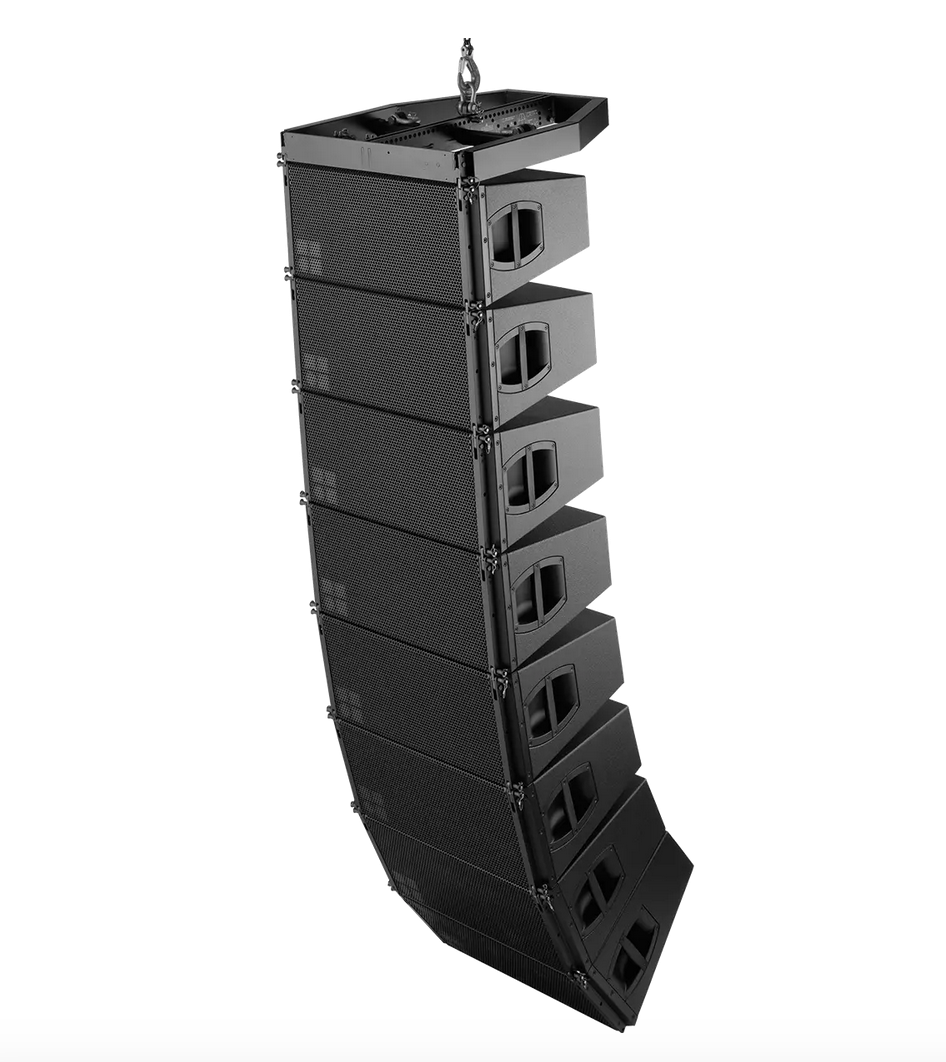
\includegraphics[width = 0.4\linewidth]{figs/dbAudiotechnik.png}
            \caption{D\&B Audiotechnik V12 loudspeaker line array.}
            \label{dbAudiotechnik}
        \end{figure}

        Another example of sound field control, this time more commonly found indoors, is wave-field synthesis, where arrays of loudspeakers are used to simulate wavefronts from virtual acoustic sources propagating through a set area.

        The defining characteristic of the wave-field synthesis technique is that the virtual acoustic sources do not change position in relation to an observer moving throughout the field, and may be placed such that the sound `radiating' from each source can come from anywhere within the field.
        This allows wave-field synthesis to become an incredibly powerful tool of sound field control, and as such the design of loudspeakers used in wave-field synthesis techniques is of note.


    \section{Loudspeaker Construction}
        Loudspeakers are typically constructed within a `cabinet', that is, an enclosure that prevents the rear radiation of a loudspeaker from destructively interfering with the frontal, on-axis radiation.
        These cabinets come in a variety of forms: Sealed, vented, transmission line or, in the case of multi-driver cabinets, a combination of any of the aforementioned.
        When mounted in a cabinet, the rear radiation from a driver does not simply disappear, it instead interacts with the acoustic environment present inside the cabinet.

        \begin{figure}[H]
            \centering
            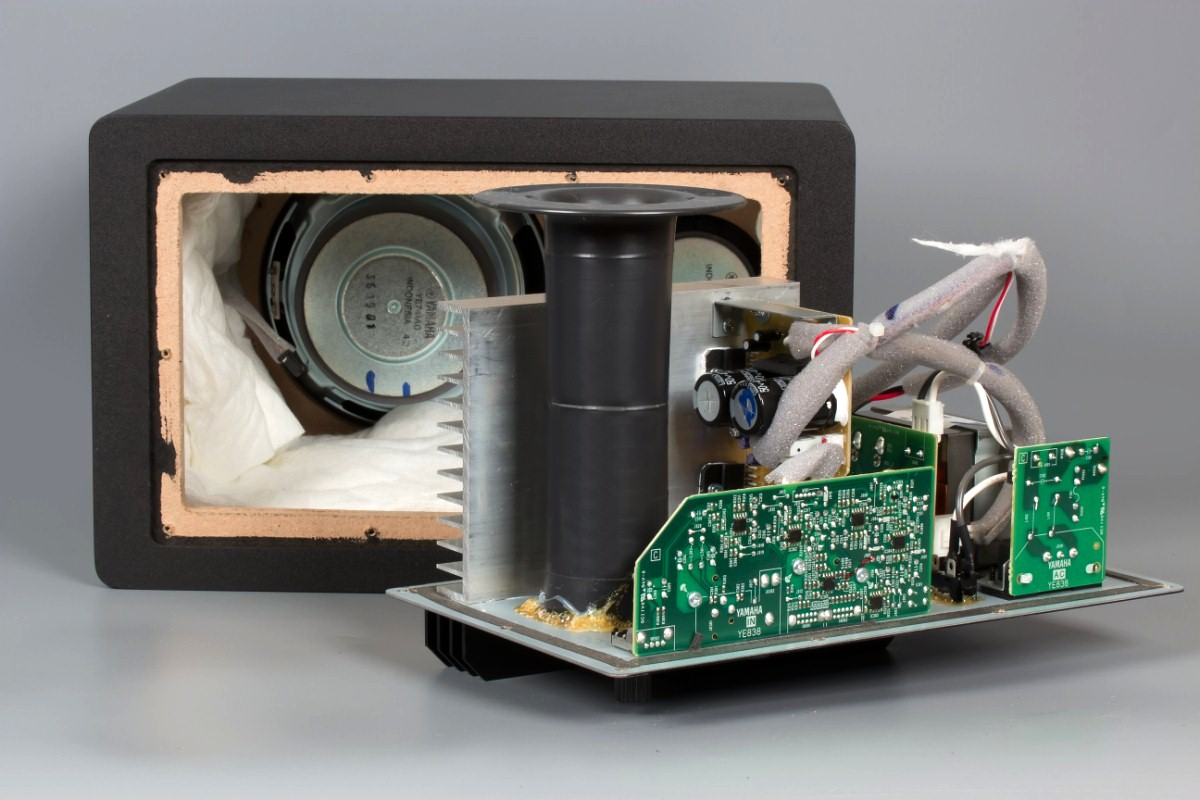
\includegraphics[width = 0.6\textwidth]{figs/hs-7back.jpg}
            \caption{A deconstructed Yamaha HS7 studio monitoring loudspeaker, note the acoustic treatment inside the cabinet and the embedded DSP chips on the printed circuit board \cite{ASRcrosssection}.}
            \label{hs-7back}
        \end{figure}

        Figure \ref{hs-7back} shows how manufacturers will use acoustic treatment to manipulate the acoustic interactions between the rear radiation of the driver and the cabinet.
        The construction of the prototype ACL follows this general scheme, and is constructed with a sealed cabinet.
        A sealed, cylindrical, perspex cabinet with plywood reinforcements houses the two low frequency (LF) drivers.
        This cabinet is then stuffed with fibrous acoustic treatment to damp any standing waves that may occur within.

        Coaxially mounted to the front face of the cylinder is a KEF Uni-q coaxial driver with a 3D-printed waveguide.
        Coaxial driver configurations are a design choice that leads to axisymmetry in driver directivity, that is, the driver may be rotated about the axis of coaxial mounting and no phase shift between woofer and tweeter at the crossover point will be introduced, as the distance between the listener and both drivers remains constant.

        Each driver in the unit requires it's own dedicated amplifier channel.
        This configuration, as opposed to a passive crossover, is becoming more and more prevalent as cheap, low THD and compact class-D amplifiers and DSP (filtering) chips allow multiple amplifiers to be built in to a loudspeaker unit's enclosure, allowing an input to be digitally crossed-over at the input stage for each driver before the amplification stage.
        However, none of this integrated amplification or crossover functionality is built in to the ACL.
        Instead, the ACL simply receives raw amplified input to each driver.
        The Uni-q mid-high driver requires a cross-over before testing however, as excessive LF input may damage or introduce non-linearity to the driver's response.

        Loudspeaker systems aiming to achieve good power efficiency at low frequencies will often employ a vented design.
        This is where a tuned, often cylindrical vent (as seen in Fig. \ref{hs-7back}), is mounted to a wall of the cabinet allowing air and thus acoustic pressure waves to flow out of the cabinet in a controlled manner.
        The tuning of the vent will encourage the pressure radiation from the vent to be in-phase with frontal radiation of the driver such that low-frequency response is boosted instead of destructively interfered with like in a loudspeaker hanging in free space.
        Another way of extending low-frequency efficiency is to employ a passive radiator, which is a loudspeaker diaphragm with no attached voice coil nor magnet; they cannot directly receive nor reproduce an amplified signal.
        Instead,the acoustic pressure generated by another driver in a shared, sealed cabinet in which both the radiator and the driver are mounted in, excites the diaphragm of the passive radiator and causes pressure radiation from the radiator away from the cabinet.

        \begin{figure}[H]
            \centering
            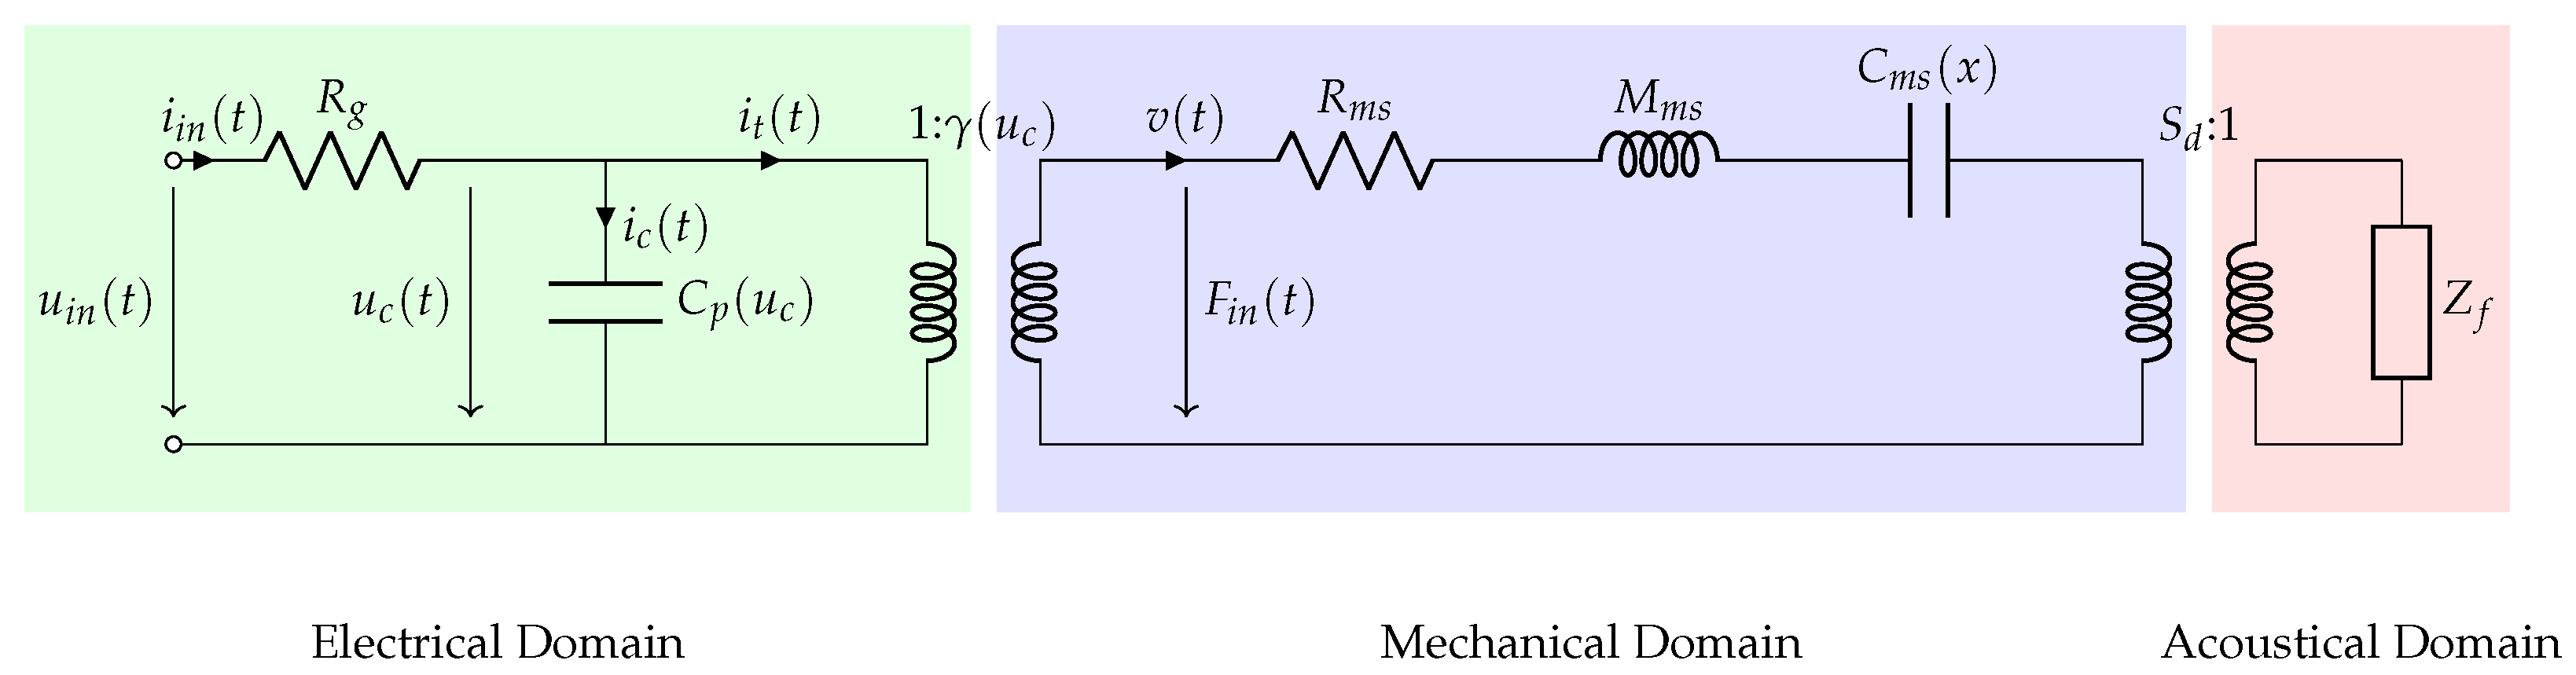
\includegraphics[width = \textwidth]{figs/equivalentCircuit.png}
            \caption{Electrical, mechanical and acoustic elements within a loudspeaker system can be represented in an equivalent circuit form \cite{liechti2021total}.}
            \label{equivalentCircuit}
        \end{figure}

        The ACL is in fact not purely any of the aforementioned configurations, instead it leans mostly towards a passive radiator based design, with two \textit{active} drivers mounted within a shared, or acoustically coupled, enclosure.
        Contrary to this, most multi-driver loudspeakers will have each active driver mounted in acoustically sealed and separate chambers.
        This design choice for the ACL is based on contemporary research which will be elaborated upon in the literature review.

        The length of the cylindrical coupled enclosure is set to 0.63 meters, shown in Fig. \ref{speakerDiagram}.
        This corresponds to a quarter-wavelength of 139Hz, which is significant as this distance between a pair of loudspeaker drivers, as is demonstrated by Harry Olson, allows for a 180-degree phase relationship between the front and rear LF drivers \cite{olson1973gradient}.
        This, theoretically, should give perfect cancellation, however real-world testing will show that it is not this simple.

        The shape of a loudspeaker enclosure and where a driver is mounted in this enclose may have an effect on the performance of the loudspeaker.
        Olson's paper `Direct Radiator Loudspeaker Enclosures' comments on the performance on cylindrical enclosures, his findings are shown in Fig. \ref{olsonCylinder} and elaborated upon in the Literature Review.

        Whilst loudspeaker design typically employs the use of equivalent circuit analogies, as shown in Fig. \ref{equivalentCircuit}, this project does not suggest any alterations to the physical construction of the loudspeaker system and as such the equivalent circuit of the system is of note, but not particularly relevant to this report.
        \newpage
    \section{General Loudspeaker Directivity}
        Understanding the directivity of a loudspeaker is a crucial component of evaluating it's real-world performance.
        Whilst sound sources are often abstracted as monopoles or dipoles with perfectly spherical radiation, in the real world the directivity of a source is much more complex and depends on many factors.
        
        The frequency component of radiated sound is one factor; low-frequency radiation is typically modelled as monopole and high frequency radiation from a loudspeaker often shows `lobing', as can be seen in Fig. \ref{initialDirectivity}.
        This relationship is due to the negative proportionality between wavelength and frequency, where wavelengths get shorter the higher a signal's frequency increases.

        A common method of measuring the directivity of a loudspeaker is to calculate a directivity factor.
        Equation \ref{directivityFactor} shows how the directivity factor, as a function of frequency, is simply a ratio of radiated sound intensity from a measured loudspeaker $I_r$ to the sound radiated from a monopole point source \cite{meggitt2020loudspeakers}.
        This factor is then converted in to a decibel scale for ease of understanding.

        \begin{equation}
            \begin{split}
                Q(f) &= \frac{I_r}{I_p} \\
                DI(f) &= 10\log_{10}(Q(f))
                \label{directivityFactor}
            \end{split}
        \end{equation}
        
        Controlling the directivity of a loudspeaker may be achieved first with the physical design of a loudspeaker, the three-dimensional waveguide surrounding the Uni-Q on the ACL is a good example of this.
        However, manipulating the phase relationship between arrays of multiple loudspeaker drivers is also a prevalent method, and is the method explored in this project.

        By introducing a phase shift between two acoustic point sources that have some spacing apart, the zones of constructive and destructive interference can be manipulated such that the combined `beam' of radiated sound can be steered.
        This, and other multi-driver directivity control theory, was pioneered by Harry Olson, and Olson's work will be elaborated upon in the literature review.

        \begin{figure}[H]
            \centering
            \hspace{2.5cm}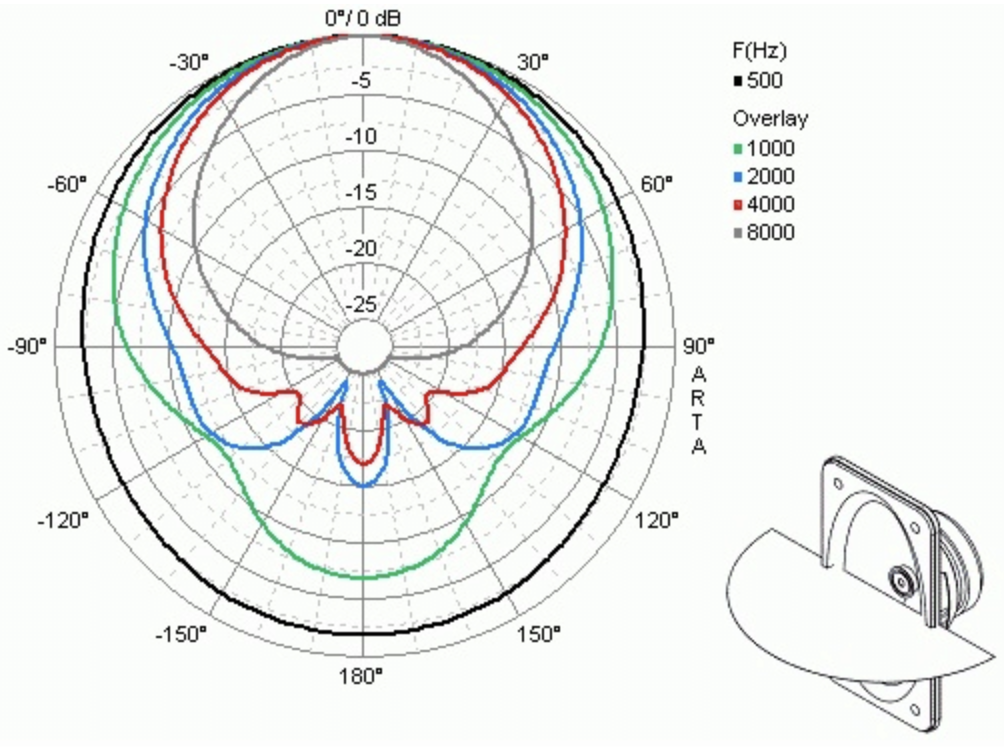
\includegraphics[width = 0.7\linewidth]{figs/generalDirectivity.png}
            \caption{Directivity plot of Visaton WB 10 loudspeaker \cite{samarasinghe2016room}.}
        \end{figure}
        
        \newpage
        
    \section{Spherical Harmonics}
        The theory behind spherical harmonics is an extension of Fourier analysis into the domain of three-dimensions and in particular, the surfaces of spheres.
        This is relevant to the directionality of a loudspeaker, as acoustic waves propagating from a monopole source, such as low-frequency radiating loudspeaker, are generally spherical \cite{kinslerFreySpherical}.
        As such, the theory of spherical harmonics was chosen to characterize and measure the directivity of the ACL.

        It is important to note the co-ordinate system used to characterize spherical harmonics in this report, Fig. \ref{sphericalCoords} illustrates this system.
        The polar angle $\beta$ is of particular note when used to derive a metric of cardioid directivity.
    
        \begin{figure}[H]
            \centering
            \begin{minipage}{.4\textwidth}
                \centering
                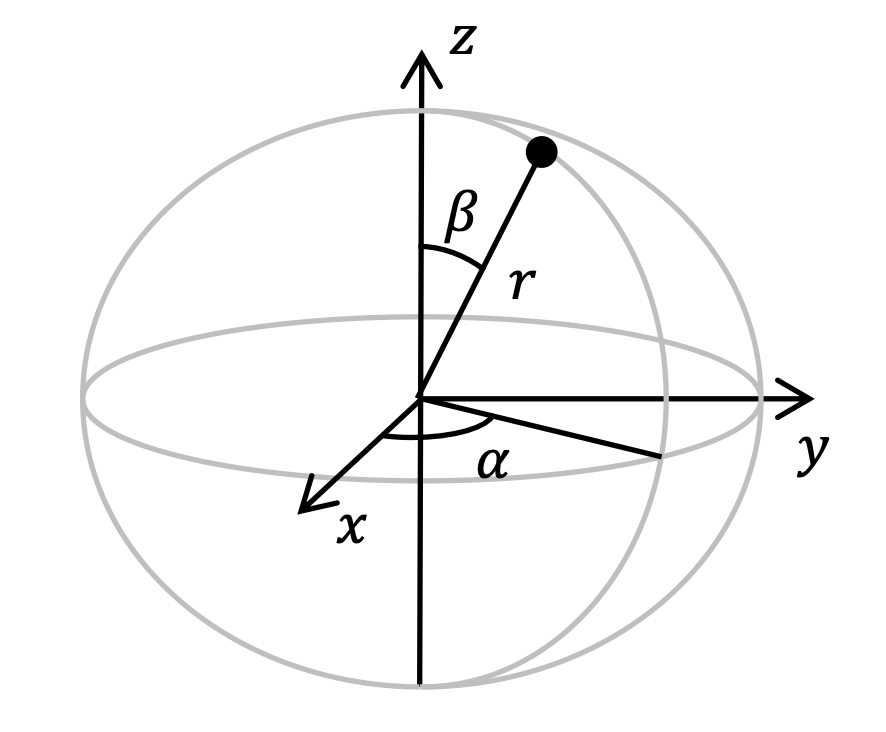
\includegraphics[width=\linewidth]{figs/sphericalCoords.png}
                \caption{Spherical harmonic coordinate system \cite{hargreaves2020spherical}}
                \label{sphericalCoords}
            \end{minipage}
            \begin{minipage}{.59\textwidth}
                \centering
                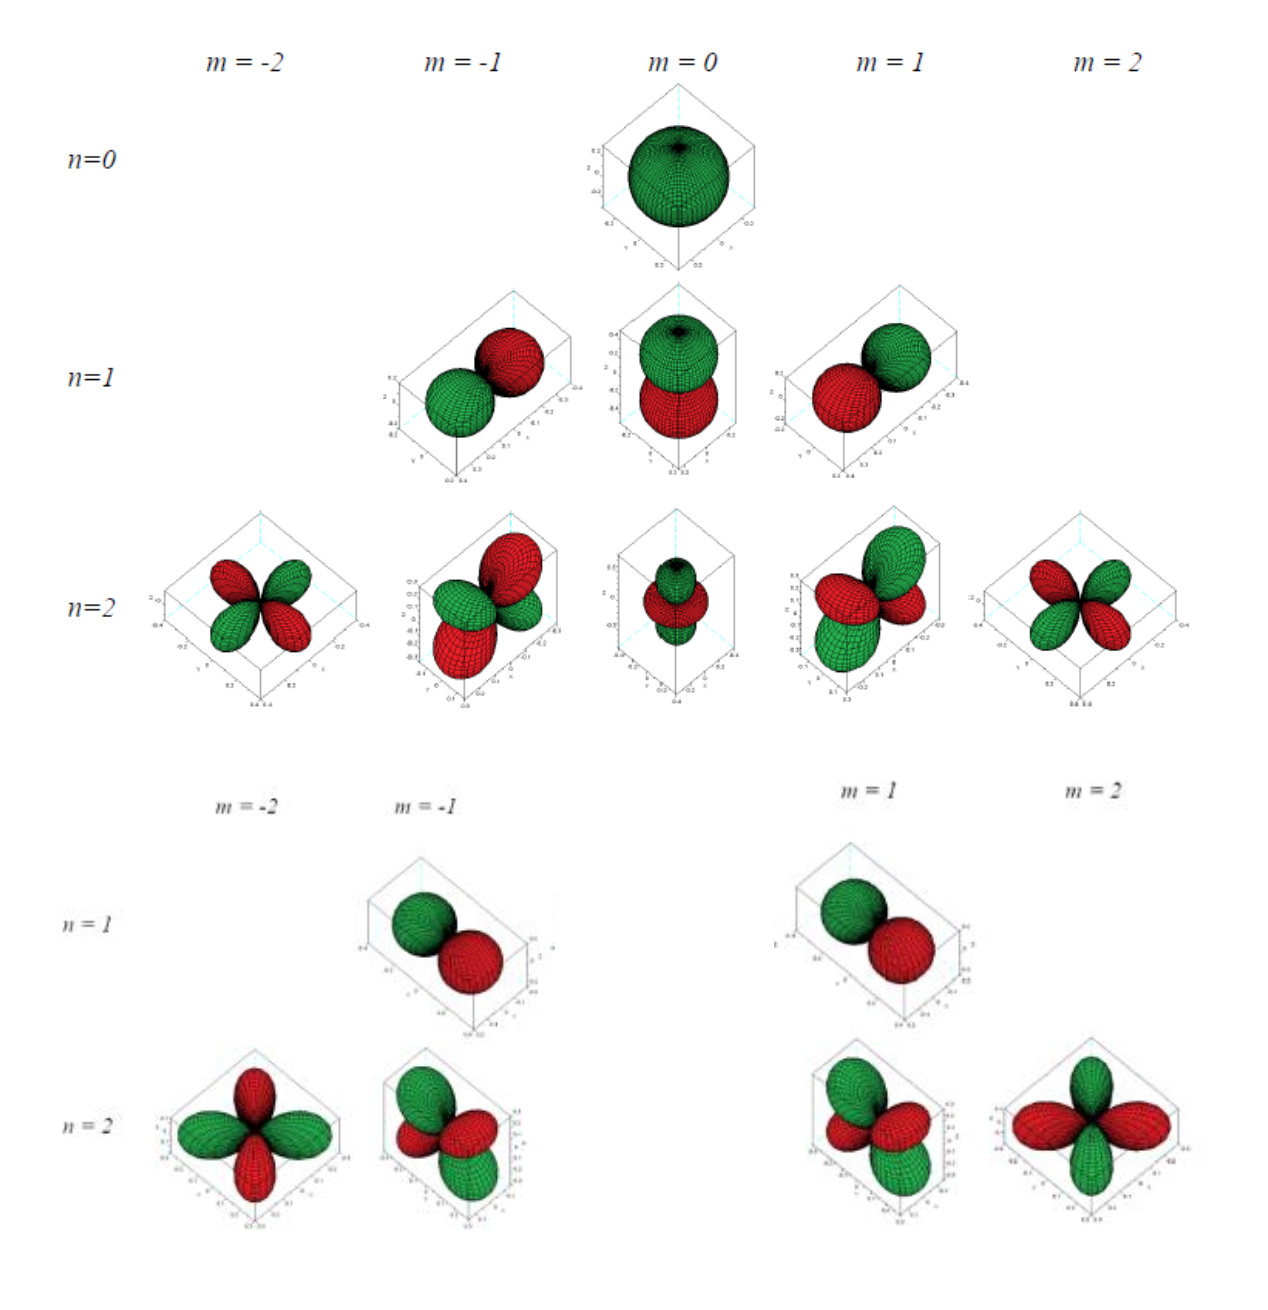
\includegraphics[width=\linewidth]{figs/klippelSphericalHarms.png}
                \caption{Ascending orders of real-valued spherical harmonics \cite{klippel2016holographic}.}
                \label{klippelSphericalHarms}
            \end{minipage}
        \end{figure}

        The lowest zero-order spherical harmonic, shown in Fig. \ref{klippelSphericalHarms}, describes the behavior of sound waves emanating from a single point source (a monopole).
        Next, the first-order spherical harmonic describes the behavior of two opposite sources with the same strength and frequency (a dipole).
        Higher order harmonics can account for more complex sound sources and reflectors, such as spherical resonators and the scattering from diffusers, however these harmonics are not considered when characterizing the directivity of the ACL.
        Discarding the higher-order harmonics will allow for easier mathematical analysis of the system, but will also lead to a less accurate characterization.

        
        A metric was ultimately derived from functions of the zero and first order spherical harmonics by a previous master's student at the University of Salford, this will be elaborated upon in the literature review.

    \section{Digital Filtering}
        Digital filters are commonplace found in the modern world of audio processing, whether in software, prototyping, or embedded systems.
        Digital signal processing (DSP) as a discipline has been prevalent since the 1960s, prominent textbooks on DSP include Alan. V. Oppenheim and Ronald Schafer's `Digital Signal Processing' \cite{oppenheim1975digital} and Francis Li and Trevor Cox's `Digital signal processing in Audio and Acoustical Engineering' \cite{li2019digital}.
        The filtering techniques used in the project described by this dissertation are derived from these textbooks.

        The digital filtering performed in this project would be within the real-world framework of an embedded system, where firmware on a digital signal processing (DSP) chip, such as an Analog Devices SigmaDSP®, are used to process some input to a system, which is a loudspeaker unit this case.
        However, as a work-in-progress prototype, all filtering is contained within MATLAB scripts used to output test signals to each driver.

        This style of embedded filtering is often found within loudspeakers that may have to work with design constraints like portability or ruggedness.
        However, signal processing is also used within high-budget, professional-level systems deployed at large-scale events.
        In this case, DSP may be used to cross-over loudspeaker units into their dedicated frequency bands or introduce time-based delay to delay lines at an outdoor event.

        An audio filter will generally have some amplitude-over-frequency response and some phase-over-frequency response.
        Filters need not have both of these characteristics, they may have a totally flat frequency response but a specific phase response (`all-pass filter'), and a filter may also have a precise frequency response and a totally linear phase response.
        In the digital domain an audio signal is represented by a sequence of discrete samples of an analog voltage both in the frequency and time domains.

        Audio filtering in DSP may at times be analogous to audio filtering in the domain of analogue electronics, where components with `memory' dictate the characteristics of a filter. 
        In analogue electronics, these components are capacitors and inductors, and their `memory' is the time taken to charge and discharge.
        In the context of DSP, the `memory' of a filter is found in delay lines or `taps' and their time-domain response to a unit impulse, or, the `impulse response' of the filter.
        In order to implement a digital filter to the time-domain form of a signal, a discrete-time convolution must be performed between the signal and the impulse response of the filter.
        Digital filters are described and implemented using $a$ and $b$ coefficients.

        \begin{figure}[H]
            \centering
            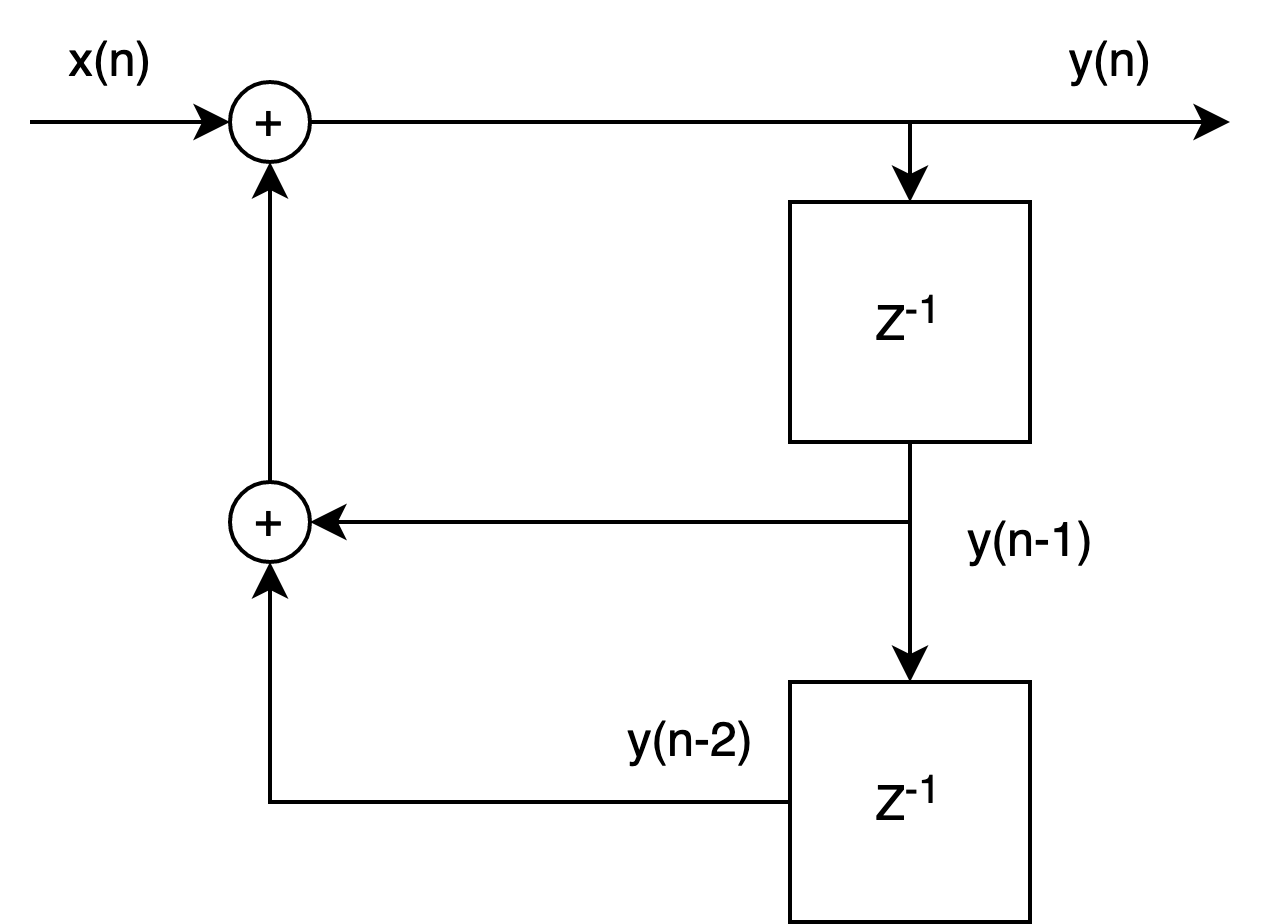
\includegraphics[width = 0.4\linewidth]{figs/filterGraph.png}
            \caption{A two-tap digital filter, represented in a signal flow chart.}
            \label{filterGraph}
        \end{figure}
        
        In this project, a finite impulse response (FIR) filter is derived in order to fit a certain frequency and phase response required at the rear driver such that the combined response of the front and rear driver is cardioid.
        A FIR filter is named over the fact that it's time-domain impulse response is finite-length and eventually decays to zero \cite{litwin2000fir}.
        The length of the FIR filter's impulse response corresponds to the number of filter taps, determining the filter's order.
        FIR filters have no $a$ coefficients, instead only having $b$ coefficients.
        The samples in the impulse response of the FIR filter \textit{are} the $b$ coefficients of the filter.
        To implement the FIR filter, simply convolve the impulse response with the time-domain signal you wish to filter.
        
        The discrete-time convolution equation used to perform the convolution operation in the digital domain is listed in Eq. \ref{convolution}.
        A property of use in this project is that convolution in the time domain is equal and reciprocal to multiplication in the frequency domain.
        The methodology section of this report will elaborate on the use of an FIR filter in this project, and the results of the derived filter.

        \begin{equation}
            y[n] = x[n] * h[n] = \Sigma_{k=-\infty}^{+\infty} x[k]h[n-k] \cite{oppenheim1975digital12}
            \label{convolution}
        \end{equation}

        Of particular note is the causality of the filter.
        In DSP, causality refers to the relationship between the input and output signals of a system.
        A causal filter is one in which the output at any given time is dependent only on past and current input values, and not on future input values.
        In other words, the output of a causal filter can only be affected by events that have already occurred, and not by events that will occur in the future.
        It is necessary for filters to be causal in order to be physically realizable; a system cannot look into the future.
        However, mathematical derivations of filters using commonplace techniques may lead to an anti-causal impulse response

        A causal filter can be implemented using a variety of digital filter structures, such as finite impulse response (FIR) filters or infinite impulse response (IIR) filters.
        FIR filters are inherently causal, as they rely only on past and current input values to generate their output.
        IIR filters, on the other hand, may be non-causal, depending on their implementation; it is from this possibility of non-causality that designing an IIR filter to fit the complex frequency response found in $\gamma$, the filter derived in this project, becomes impractical. 

        When a causal filter is applied to a signal, the filter introduces a delay in the output signal relative to the input signal.
        This delay results in a phase shift in the time domain, which may or may not be beneficial, according to the design specification of the filter.
        This phase shift may be particularly pronounced in FIR filters, which introduce a linear phase shift that is proportional to the filter's delay, due to the delay-line nature of their construction.

        \begin{figure}[H]
            \centering
            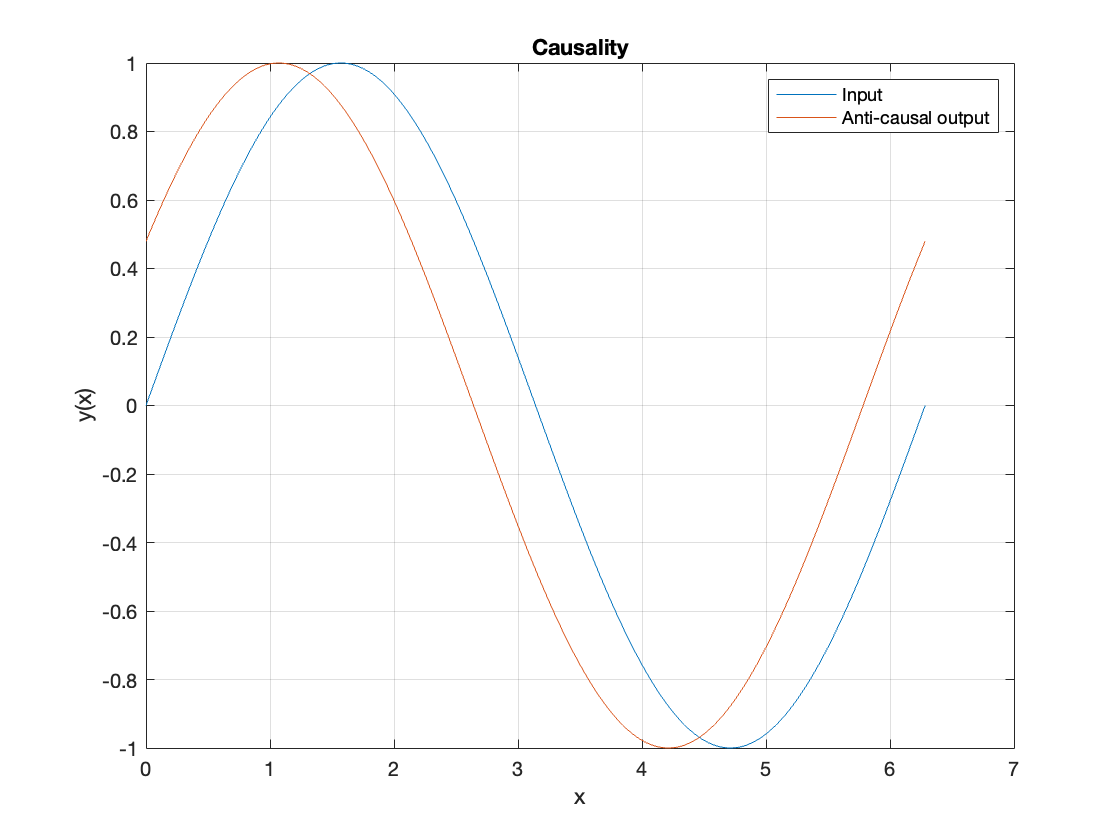
\includegraphics[width = 0.5\linewidth]{figs/causality.png}
            \caption{An anti-causal output will be in negative time compared to the input.}
            \label{causality}
        \end{figure}
        
        A notable property of FIR filters is that the impulse response can extend infinitely into the future, or more precisely, it can wrap around from the end of the sequence to the beginning.
        This wrapping around is an important property in FIR filter design, as it allows us to treat the impulse response of an FIR filter as a circular buffer.
        This allows for a more efficient convolution of the FIR filter with an input signal, as opposed to convolving a large, unwieldy impulse response with every sample block in a digital audio buffer.

        
\chapter{Literature Review}
    \section{Investigations into the Use of Loudspeakers in Sound Field Control}

        Indoor sound field control techniques are explored by Ole Kirkeby and Philip A. Nelson in `Reproduction of Plane Wave Sound Fields' \cite{kirkeby1993reproduction}.
        In particular, Kirkeby and Nelson investigate how well a plane wave may be reproduced by an array of monopole sources suspended in a free field.
        Ultimately they found that the quality of a generated plane wave sound field is tied to the angles between each source and the center of a receiver array and the size of the receiver array.
        These conclusions were reached by applying the Kirchoff-Helmholtz theorem to a continuous two-dimensional plane over which a sound field is controlled \cite{kirkeby1993reproduction}.
        This work can be related to the technique of wave field synthesis.

        `Sound Field Control with a Circular Double-Layer Array of Loudspeakers', by Ji-Ho Chang and Finn Jacobsen makes a key point regarding sound field control with loudspeakers: That the methods described in literature may be separated into those that seek to approximate a desired sound field, and those that seek to create acoustic `dark' and `bright' zones \cite{chang2012sound}.
        In other words, loudspeakers can manipulate the sound within a zone, facilitate sound field control which aims to exclude or encourage the presence of sound in particular zones.
        They further elaborate on a method which seeks to synthesize the aforementioned categories and control wavefront behavior, like in Kirkeby and Nelson's paper, whilst maintaining an acoustic dark and bright zone.

        \begin{figure}[H]
            \centering
            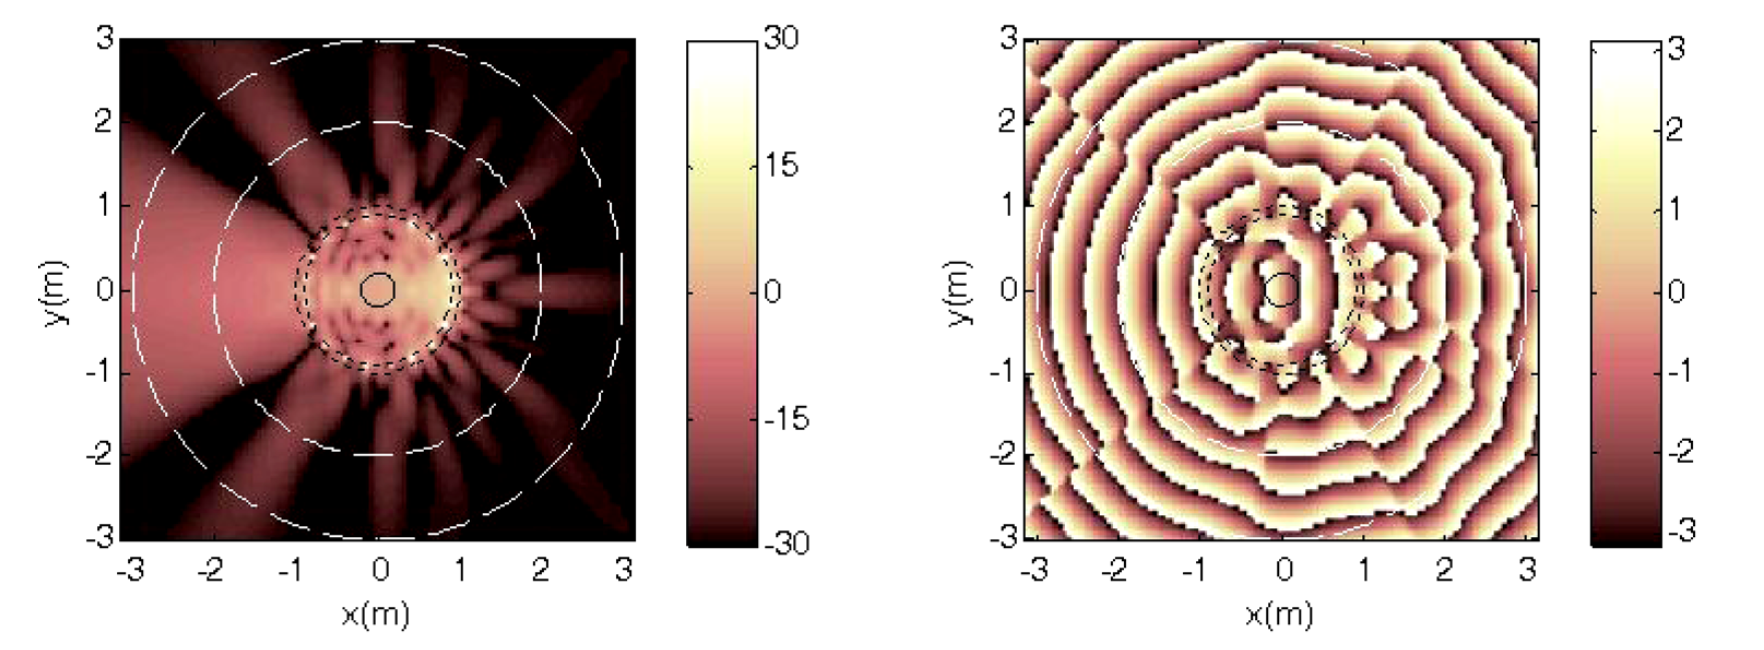
\includegraphics[width = 0.6\linewidth]{figs/changField.png}
            \caption{Simulations show Chang and Jacobsen's circular array manages to both recreate a plane wave within the sound field \textit{and} create a acoustic bright and dark zones \cite{chang2012sound}.}
            \label{changField}
        \end{figure}

        Whilst the findings of this paper were obtained through simulation, it is worth noting that Chang and Jacobsen specify the simulated loudspeakers used.
        Individual loudspeakers in the array are modeled as a weighted combination of a dipole and a monopole, with cardioid directivity.
        As a two-layer circular array, the innermost layer of loudspeakers points toward the center of the bright zone, and the outer points away.
        This use of cardioid loudspeakers suggests suitability of the ACL for a real-world recreation of this array, albeit the length of a cylinder-based design may make a two-layer configuration unwieldy.

        Franz M. Heuchel, Diego Caviedes-Nozal, Jonas Brunskog, et al. explore outdoor sound field control in their paper: `Large-scale outdoor sound field control' \cite{heuchel2020large}.
        The authors investigate the low-frequency directivity performance of loudspeaker systems across atmospherically varying outdoor spaces, as opposed to the linear, homogenous, and isotropic conditions often assumed indoors.
        This paper contains many points of interest for this project, beginning with employing Kirkeby and Nelson's pressure matching method \cite{kirkeby1993reproduction} to derive an optimal filter to apply to the `control' loudspeakers providing the active cancellation that gives a zone of sound field control.
        This optimal filter is generated using the inverse fast Fourier transform method (IFFT), the same technique as is used in this ACL project.
        
        Spherical harmonics are also employed to create a sound propagation model, in which the generating loudspeakers are assumed to be axisymmetric.
        However, the spherical harmonics used are of a higher order than those utilized in this project. 
        Heuschel et al. use Jacobsen and Juhl's model for expressing sound propagation in spherical coordinates, seen in Eq. \ref{heuchelSpherical}.
        
        \begin{equation}
            \hat{h}(\matr{r},\matr{a}) = \Sigma_{m=0}^{M}a_m h_m^{(2)}(kr)P_m(\cos(\theta)) \cite{jacobsen2013fundamentals}
            \label{heuchelSpherical}
        \end{equation}

        Ultimately Heuchel, Caviedes-Nozal, Brunskog, et al. find that using active control systems is effective in sound field control in large outdoor environments, but note that varying meteorological conditions must be accounted for in real time, as expected.
        More importantly, their work involves the use of a loudspeaker specification and directivity measurement that is very close to that which is investigated in this project.

    \section{Historical Directional Loudspeaker Designs}

        Harry Olson's `Gradient Loudspeakers'~\cite{olson1973gradient} forms the theoretical foundation of controlling the directionality of emitted sound with multiple loudspeaker drivers.
        The key concept Olson introduces is the `gradient loudspeaker', which are organized into orders.
        Zero-order gradient loudspeakers utilize a single driver within a sealed cabinet to give a theoretical monopole directionality, much like an omnidirectional microphone.
        Higher orders introduce directionality; a first-order unidirectional loudspeaker constructed with a spaced and delayed pair of zero-order gradient speakers operating 180\degree\@ out of phase gives a cardioid response.
        The delay between both drivers is fixed across all frequencies.
        Olson gives the radiated pressure of this unidirectional gradient loudspeaker, shown in Eq.\ref{olsonFirstOrderPressure}.

        \begin{equation}
            p = 2CU_f\cos{kct}[\sin{\frac{kd}{4}+\frac{kD}{4}\cos{\theta}}]
            \label{olsonFirstOrderPressure}
            \cite{olson1973gradient}
        \end{equation}

        \begin{figure}[H]
            \centering
            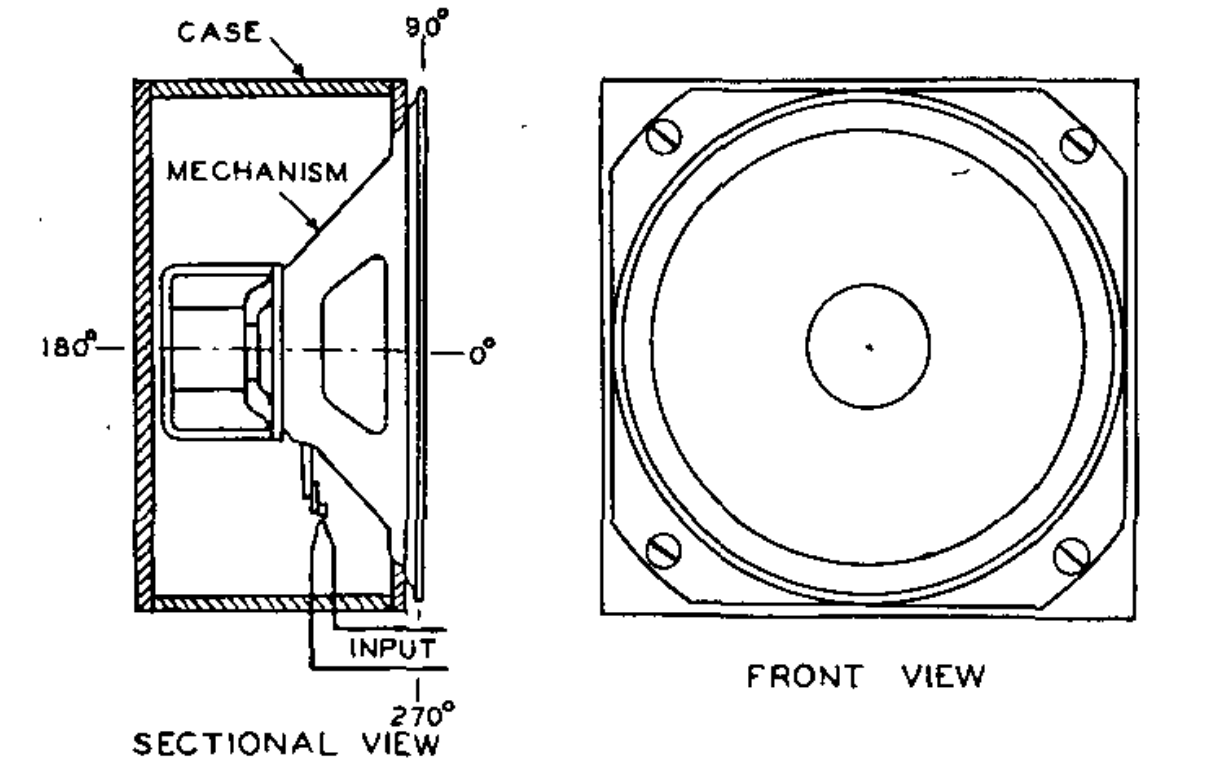
\includegraphics[scale=0.4]{figs/olsonFirstOrder.png}%
            \caption{Olson's first order unidirectional loudspeaker.}\cite{olson1973gradient}
            \label{olsonFirstOrderDiagram}
        \end{figure}

        Olson states that if the distance between the drivers, $D$ equals $d$, the distance delay introduced and seen in Fig.\ref{olsonFirstOrderDiagram}, the directivity of the system will be cardioid.
        The wavenumber, $k$, found in Eq.\ref{olsonFirstOrderPressure}, introduces a frequency dependence to the $D=d$ condition.
        Figure \ref{olsonFirstOrderDirectivity} shows that across a range of frequencies, a cardioid polar pattern is maintained, albeit with slight differences.

        \begin{figure}[H]
            \centering
            \begin{minipage}{.4\textwidth}
                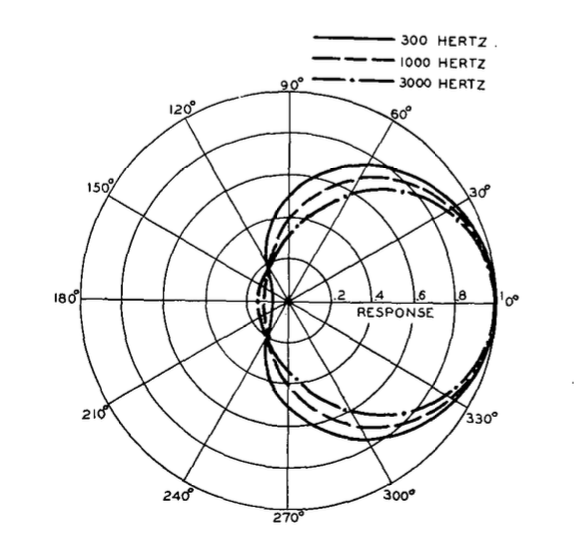
\includegraphics[width=\linewidth]{figs/olsonFirstOrderDirectivity.png}
                \caption{Directivity response of the first-order unidirectional loudspeaker.}\cite{olson1973gradient}
                \label{olsonFirstOrderDirectivity}
            \end{minipage}
            \begin{minipage}{.55\textwidth}
                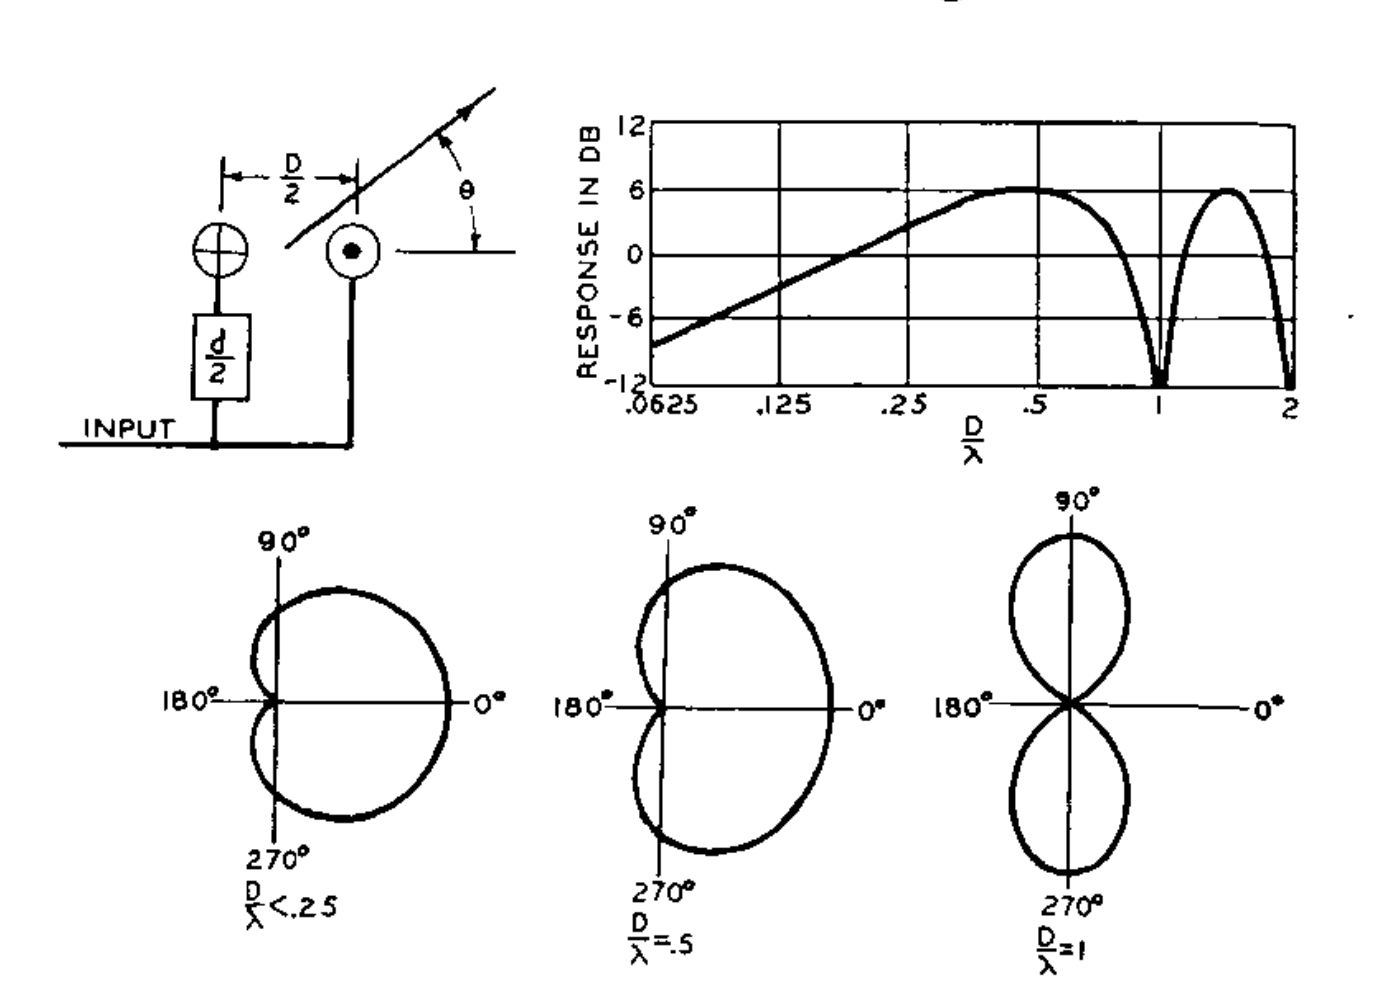
\includegraphics[width=\linewidth]{figs/olsonFreqResponse.png}
                \caption{Frequency response of the first-order unidirectional loudspeaker.}\cite{olson1973gradient}
                \label{olsonFreqResponse}
            \end{minipage}
        \end{figure}

        Note that Olson's gradient loudspeakers are the result of sums of ideal monopoles, and no real world speaker is so uniform in directivity or frequency response.
        The compensation filter outlined in this dissertation will seek to correct for the individual directivity of the LF loudspeakers through a more general analysis of the system as a whole.

        Predating his work on gradient loudspeakers, Olson was an early descriptor of the beam narrowing effect of loudspeaker line arrays \cite{olson1957acoustical}.
        Line arrays would go on to be a principle tool of sound field control in the modern day, but gradient loudspeakers are still, relative to line arrays, uncommon.
        Cardioid subwoofer systems used in live audio are common implementations of gradient loudspeaker designs.
        These subwoofers can be sold as gradient loudspeakers themselves, often with switchable directivity patterns; audio engineers will also arrange standard, omnidirectional subwoofers into configurations that introduce a phase delay sufficient to create a cardioid directivity pattern~\cite{curtis2022cardioidsubs}.
        
        Olson's 1969 paper `Direct Radiator Loudspeaker Enclosures' comments on the frequency-domain performance of a cylindrical loudspeaker cabinet construction \cite{olson1969direct}.
        Whilst this paper does not deal with explicitly directional loudspeakers, it gives a useful insight to any frequency-domain effects that may affect the phase relationship between the front and rear LF driver of the ACL.
        Figure \ref{olsonCylinder} shows a degree of comb filtering introduced above 600Hz.
        The paper also describes frequency response measurements of various other loudspeaker enclosure shapes and finds similar effects in cuboid end-fire loudspeakers, suggesting the shape of the frequency response may be related to the end-fire nature of loudspeaker driver placement within an enclosure.
        
        \begin{figure}[H]
            \centering
            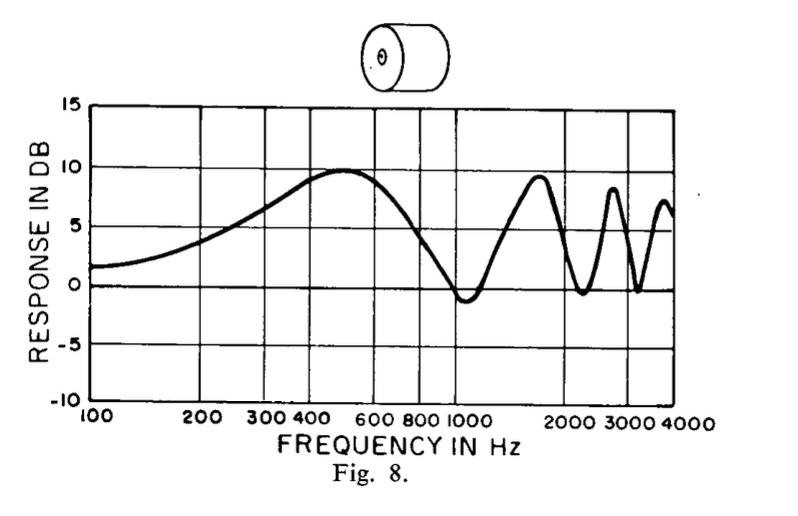
\includegraphics[width = 0.7\linewidth]{figs/olsonCylinder.png}
            \caption{Olson's testing finds the frequency response of an end-fire cylindrical loudspeaker.}
            \label{olsonCylinder}
        \end{figure}

        Olson finds that a spherical enclosure gives the least (linear) frequency-domain distortion, this may be a cabinet construction worth investigating for an ACL in the future. 

        Jordan Cheer elaborates on the use of a `two source line array', which in essence is an Olson-style directional gradient loudspeaker, stating: `Two-source line arrays have been used in a variety of applications to generate localised listening zones and have also been used as a constituent element of larger arrays to achieve sound field control more generally.'\cite{cheer2015robustness}.

        \newpage
    \section{Contemporary Directional Loudspeaker Constructions}
        The prototype ACL has each low-frequency driver mounted in a shared, acoustically coupled enclosure.
        Robustness and efficiency of an acoustically coupled two-source superdirective array, an ICSV22 paper by Jordan Cheer, elaborates on the benefits of such a shared enclosure \cite{cheer2015robustness}.
        Cheer acknowledges how a superdirective array of loudspeakers have `high sensitivity to uncertainties in the assumed response of the system', and that regularization of the powered signal driving units in an array can improve the `robustness to uncertainty'.
        
        However, he further notes that these measures may limit the directivity of a such a system; counterproductive to the designed purpose of a superdirective array.
        Robustness and efficiency thus sets out to investigate the robustness of acoustically coupled two-source superdirective loudspeaker, as opposed to the previously investigated non-interacting directional loudspeakers.
        Cheer finds, using a two-port model of loudspeaker behavior and derived simulations, that an uncoupled two-source array is `more significantly affected by response uncertainties than the coupled array', and thus the coupled array is more robust, avoiding the need for regularization.
        
        \begin{figure}[H]
            \centering
            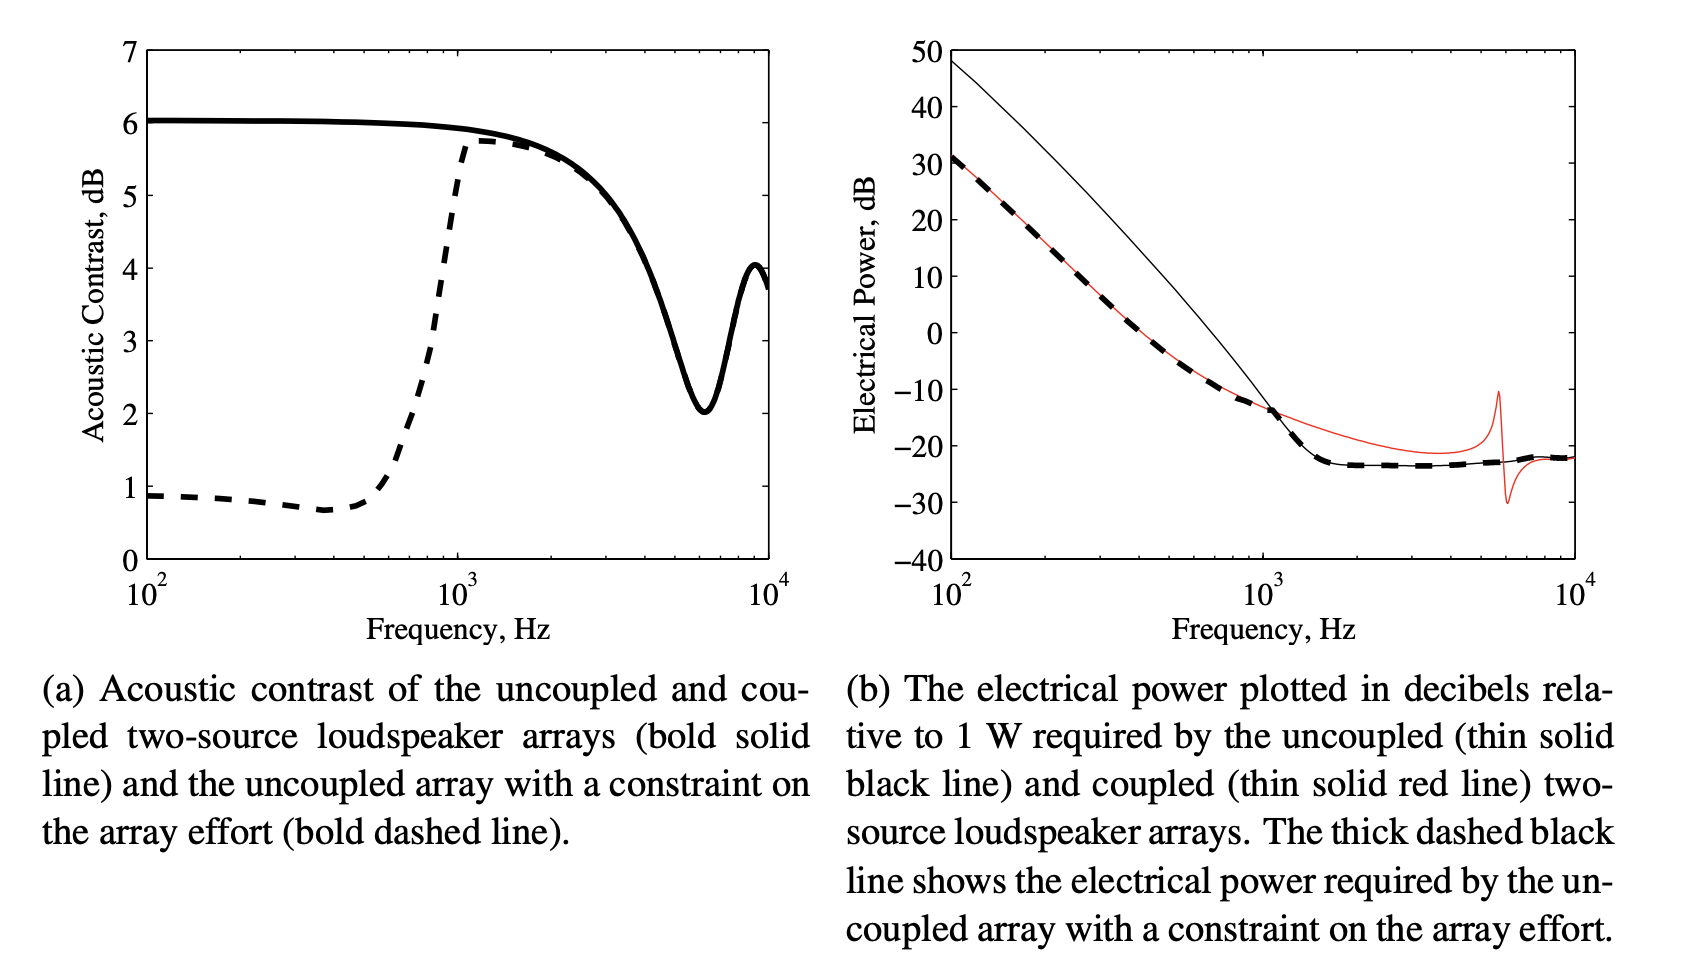
\includegraphics[scale=0.5]{figs/cheerGraph.png}%
            \caption{Cheer's plots comparing acoustically coupled and uncoupled loudspeaker systems.}\cite{cheer2015robustness}
            \label{cheerGraph}
        \end{figure}

        Cheer's figure \textit{a} (Fig.\ref{cheerGraph}) shows that when a constraint (to use the same electrical power as the coupled array) is applied to an \textit{un}-coupled two-source superdirective loudspeaker it loses a significant degree of acoustic contrast.
        Considering Cheer's findings, the ACL was constructed with an acoustically coupled main chamber for the LF drivers.

        All the drivers used in the ACL are designed by KEF and used in their commercially available products, but in different cabinet configurations to the ACL.
        However, KEF have a commercialy available ceiling-mounted loudspeaker that utilizes an LF driver with a coaxially mounted Uni-Q: The Ci250RRM-THX.
        
        \begin{figure}[H]
            \begin{minipage}{.49\textwidth}
                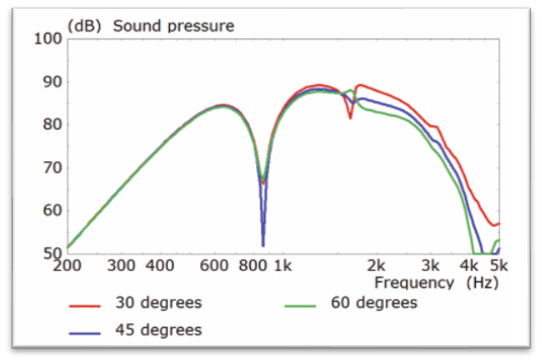
\includegraphics[width=\linewidth]{figs/KEFpressure.png}%
                \centering
                \caption{Frequency response of a LF driver with a close-back Uni-Q mounted coaxially.}
                \label{KEFpressure} \cite{KEFCi}
            \end{minipage}
            \begin{minipage}{.49\textwidth}
                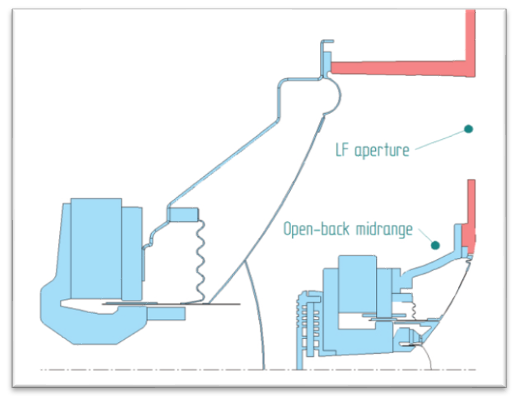
\includegraphics[width=\linewidth]{figs/KEFdiagram.png}%
                \centering
                \caption{KEF's Diagram of the Ci250RRM-THX}\cite{KEFCi}
                \label{KEFdiagram}
        \end{minipage}
        \end{figure}

        KEF found that such a three-way loudspeaker design with the LF driver mounted in a cavity to the rear of the mid-high introduces resonances, determined by the size and shape of the cavity \cite{KEFCi}.
        Figure \ref{KEFpressure} shows a dip in sound pressure between 800Hz to 1KHz; KEF remedy this by designing the Ci250RRM-THX to use an open-backed Uni-q midrange.
        KEF call this `Cavity Radiation Control', and they show, in Fig. \ref{KEFopenback}, that the 30-plus dB cancellation around 800Hz to 1KHz is eliminated.

        \begin{figure}[H]
            \centering
            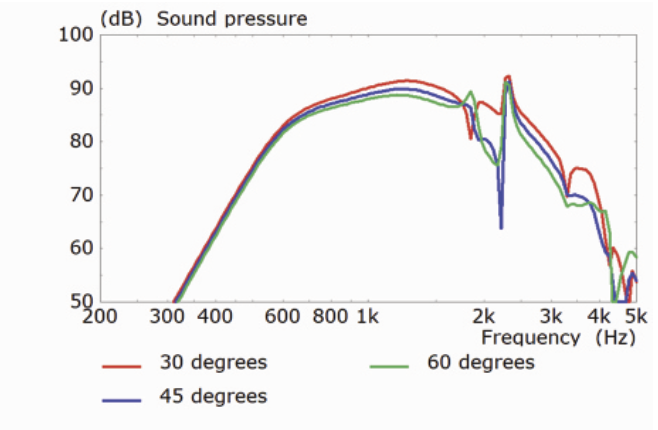
\includegraphics[scale=0.8]{figs/KEFopenback.png}
            \caption{Changing the Uni-Q to an open back design.}\cite{KEFCi}
            \label{KEFopenback}
        \end{figure}

        Whilst the model of LF driver and the cavity in which it is mounted in are different to the ACL, KEF's findings are applicable to the three-way coaxial design of the ACL and as such prompt further investigation into these `cavity resonances'.
        \newpage
    \section{Characterizing Directivity with Spherical Harmonics} 
        When describing a new, `holographic' near-field method of loudspeaker directivity measurement, Wolfgang Klippel and Christian Bellmann elaborate on the use of spherical harmonics as constituent solutions to the Helmholtz equation \cite{klippel2016holographic}.
        However, the main objective of the paper focuses on describing the holographic directivity measurement method's effectiveness at reducing the space requirements of anechoic listening environments.
        Klippel and Bellmann state that by using a spherical coordinate system the solution to the Helmholtz equation may be separated into radial and angular functions, which then form an orthogonal set of base solutions to spherical wave propagation.

        Importantly, Klippel and Bellmann, like Heuschel et al., give a spherical-harmonics based series of base solutions as an expansion of the transfer function between an acoustic input $u$, and the recieved pressure in the frequenecy domain.
        This series is given in Eq. \ref{klippelEq}.

        \begin{equation}
            H(f,\matr{r}_E) = \Sigma_{n=0}^{N(f)}\Sigma_{m=-n}^{n}C_{mn}(f) \cdot h_n^{(2)}(kr_E)Y_n^m(\theta_E,\varPhi_E)\cite{klippel2016holographic}
            \label{klippelEq}
        \end{equation}

        Hankel functions of the second kind are used in Eq. \ref{klippelEq} to describe the phase and amplitude of spherical waves propagating away from the acoustic source.
        These Hankel functions will also appear in the far-field approximations used in the project described in this dissertation.

        The project described in this dissertation builds on previous work not only by the supervisor but also by other (former) students of the University of Salford.
        During the COVID-19 lock-down period the acoustic properties and directivity of the ACL were modelled using the finite element method (FEM).
        
        Paul Vedier carried out these simulations as part of his Master's dissertation.
        A metric derived in Vedier's dissertation, is used to quantify cardioid directivity and will be utilized to achieve the practical aims of correcting for cardioid directivity over all frequencies in the ACL.
        Vedier's paper confirms, using COMSOL, that the ACL has the properties of an Olson-style gradient loudspeaker.
        In Fig.\ref{vedierPolar} Vedier compares FEM analysis of two fully-modelled membranes in a cabinet and compares to Olson's analytical method.
        
        \begin{figure}[H]
            \centering
            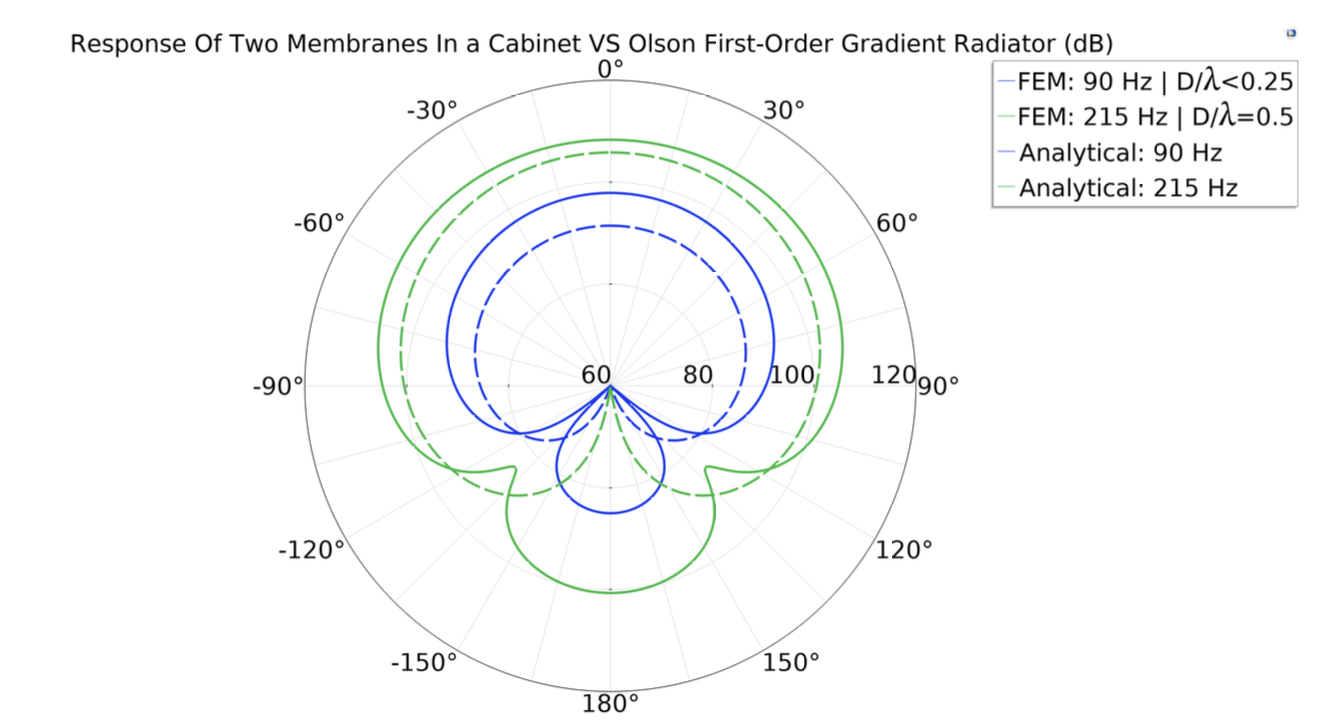
\includegraphics[scale=0.6]{figs/vedierPolar.png}
            \caption{FEM model of the ACL compared with Olson's first order unidirectional loudspeaker \cite{vedier}.}
            \label{vedierPolar}
        \end{figure}

        \newpage

        Vedier's paper describes a reduction of a series of spherical harmonic based solutions to the Helmholtz equation, like those described in Klippel and Bellmann's and Heuschel et al.'s papers.
        By accounting for anechoic conditions, an axisymmetric loudspeaker construction and far-field measurement, the zero and second order spherical harmonics were reduced to a pair of coefficients.
        The use of these coefficients to form a metric of cardioid directivity will be outlined in the methodology section of this report.
        It should be noted that Vedier's simulations did not model nor account for the coaxially mounted Uni-Q driver, so some inaccuracy to real-world performance, influenced by early reflections LF on the back of the Uni-Q's enclosure, is to be expected.

\chapter{Methodology}
    \section{Initial Transfer Function and Directivity Measurement}
        To build a numerical analysis of the directivity of the axisymmetric loudspeaker system's behavior as a whole over all frequencies, the frequency-domain transfer function of each driver must be measured across a 360-degree rotation of the $\beta$ angle shown in Fig. \ref{sphericalCoords}, where the front of the ACL is pointing in the Z-direction.
        In order to create a precise and accurate measurement free of interference and noise, the drivers were measured, assembled and mounted in their enclosures, in a fully anechoic chamber with a NTi reference-grade measurement mic.

        Ensuring the angle interval of each measurement was consistent, the loudspeaker was mounted to a Four Audio ELF robot arm which rotated the loudspeaker system about the $\beta$ angles.
        Swept sine excitation signals were fed to each driver as the input excitation.
        The output of the loudspeaker was recorded by an omnidirectional NTi measurement microphone and de-convolved from the excitation signal (recorded in a loop-back channel).
        This produced an impulse response for the loudspeaker's radiation in the anechoic chamber.
        A fourier transform of this impulse response was then taken, in MATLAB, to analyze the frequency response of the loudspeaker.

        Using swept sinusoidal waves as an input excitation for acoustic and loudspeaker measurements is an established technique \cite{loudspeakersANSI}.
        It allows for precise measurement of the entire frequency response of a loudspeaker as the sine wave input sweeps from zero hertz to the Nyquist limit.
        Sine sweeps are, however, vulnerable to environmental interference or interrupting noise throughout the duration of the sweep.
        The extreme acoustic isolation and lack of reflectivity in the anechoic chamber give good conditions for the avoidance of any such outside interference.

        Other methods of loudspeaker performance measurement exist, for example pink noise may be used as an excitation signal instead of swept sine waves. 
        Near field measurements of loudspeaker performance are also possible.
        Klippel GmbH offers a `3D Near Field Scanner' which they claim can give `Directivity, sound power, SPL response and many more key figures for any kind of loudspeaker' \cite{klippelNFS}.
        This near field scanner system also allows `holographic' spherical harmonic based directivity measurements, as outlined in Klippel and Bellmann's aforementioned paper \cite{klippel2016holographic}. 
        As aforementioned, the holographic near-field measurement technique is particularly useful when no anechoic testing environment is available; an anechoic chamber was available so this was not an issue.
        Ultimately, a swept-sine based directivity measurement technique using the Four Audio ELF robot arm was implemented.

        The two low-frequency drivers were fed by a Samson Servo-500 power amplifier, whilst the mid-high driver was fed by a University of Salford in-house made mono power amplifier, a 'Dial-a-Watt'.
        The output of the Dial-a-Watt was fed to a KEF-made cross-over, splitting the signal into mid and high frequency bands for the coaxial Uni-Q's mid and high drivers.
        The full signal flow of the transfer function measurement system is shown in Fig.\ref{signalFlow}.
        
        \newpage
 
        \begin{figure}
            \centering
            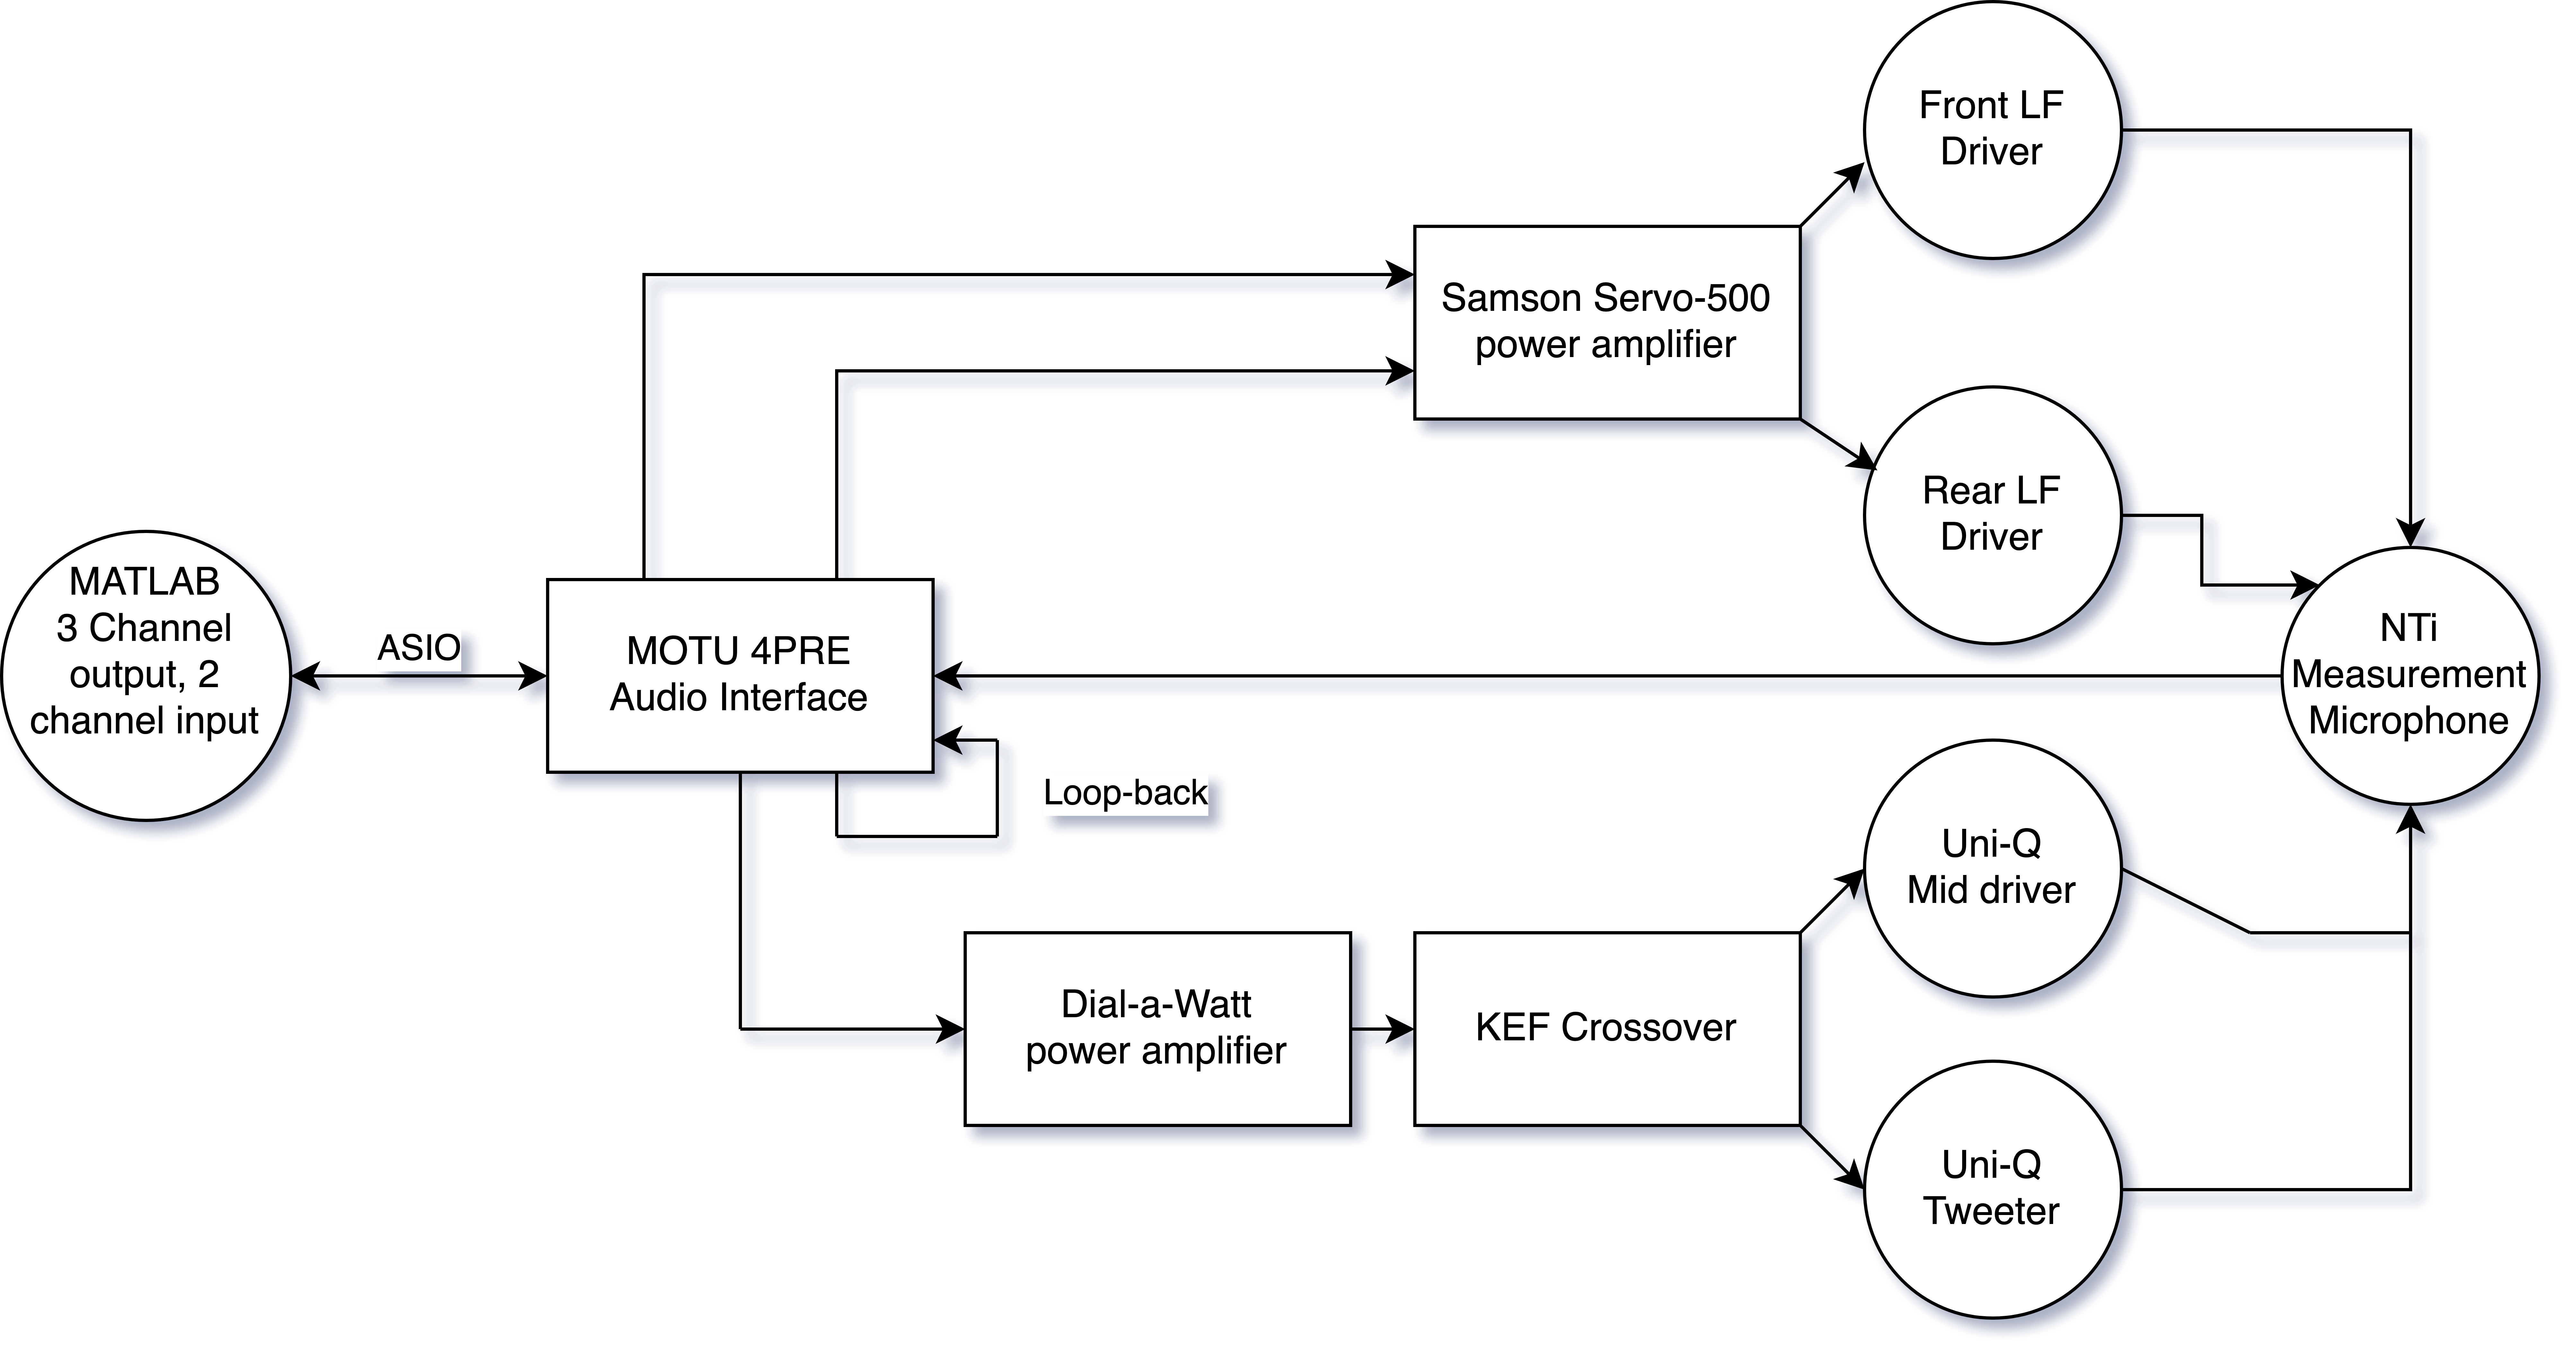
\includegraphics[width = \textwidth]{figs/signalFlow.png}%
            \caption{Signal flow of driver transfer function measurement}
            \label{signalFlow}
        \end{figure}

        \newpage

        All audio output, ELF robot arm movements and input recordings were automated through a MATLAB script, implementing API calls to the ELF robot and handling all audio buffer manipulation.

        \begin{figure}[H]
            \centering
            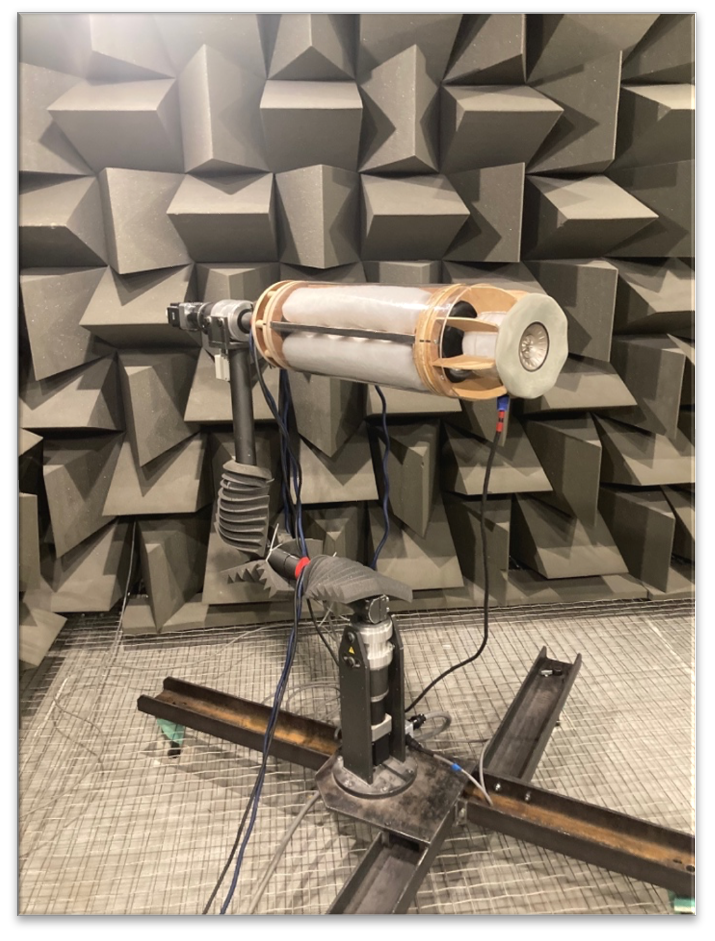
\includegraphics[width = 0.4\textwidth]{figs/speakerOnRobot.png}%
            \caption{The prototype loudspeaker mounted for testing in the University of Salford's fully anechoic chamber.}
            \label{speakerOnRobot}
        \end{figure}

        \begin{figure}[H]
            \centering
            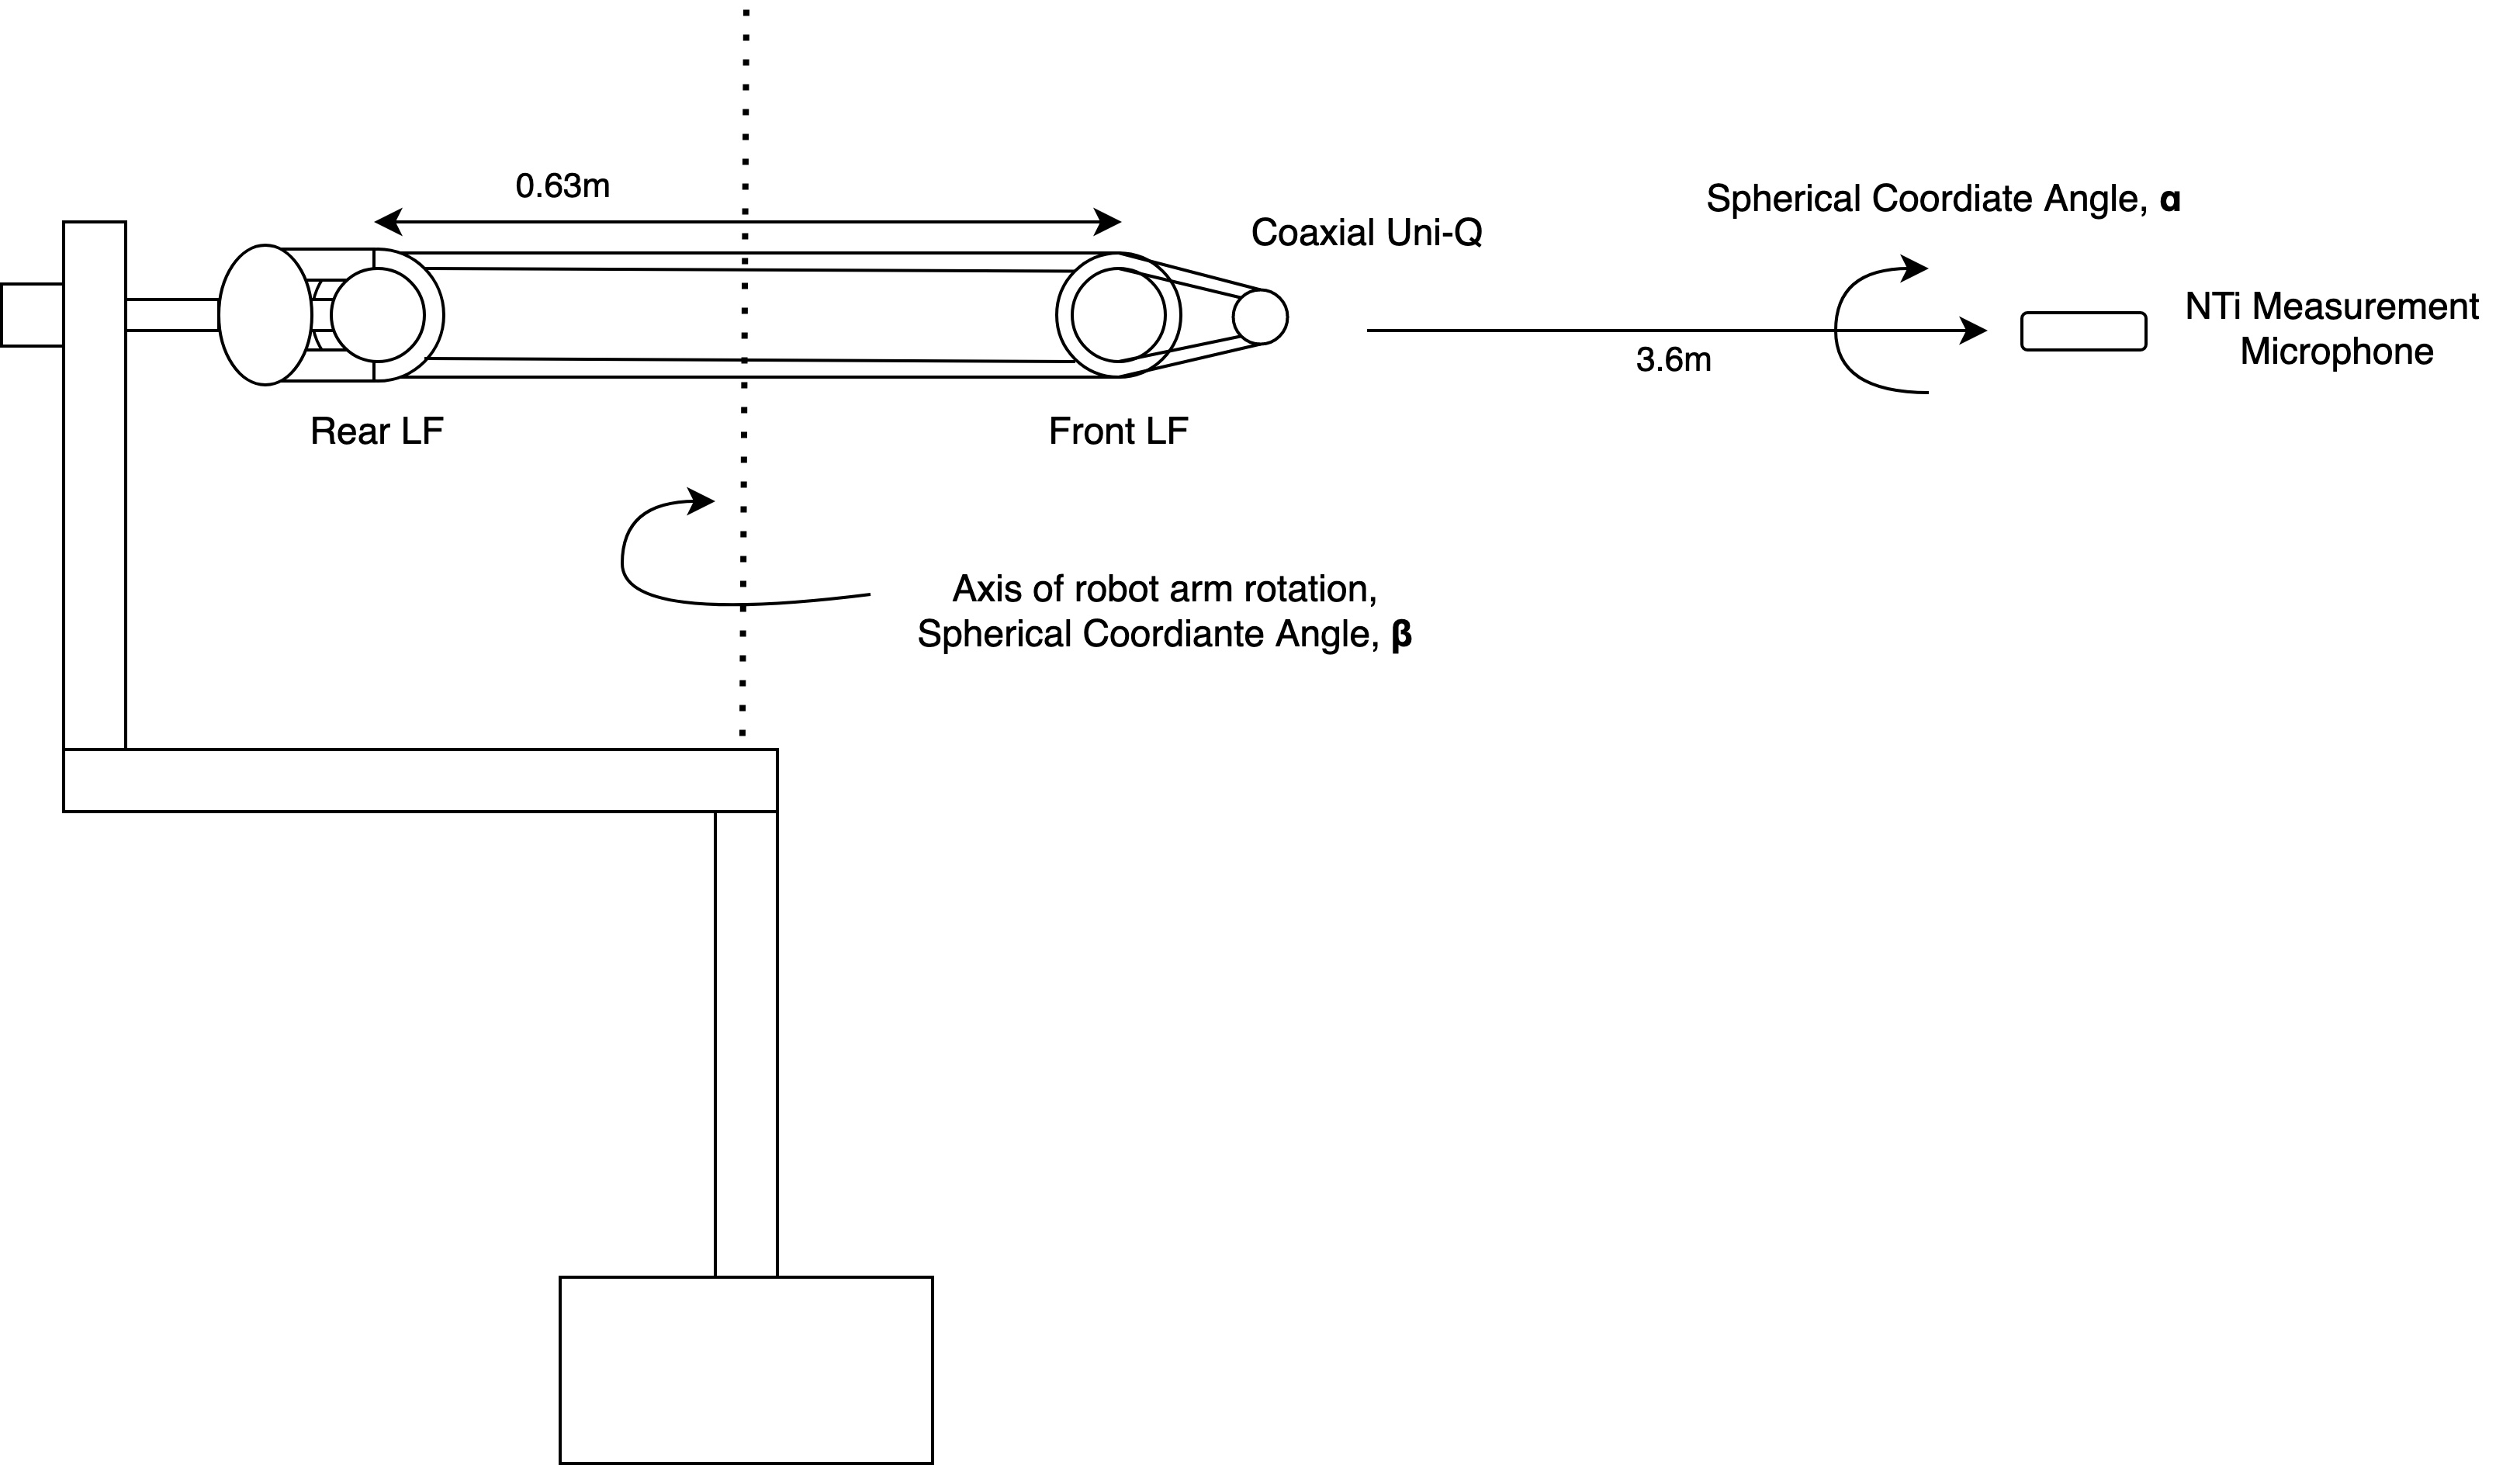
\includegraphics[width = 0.9\textwidth]{figs/speakerDiagram.png}%
            \caption{The axisymmetry of the ACL about the $\alpha$ allows for only measurements about the $\beta$ axis to be necessary.}
            \label{speakerDiagram}
        \end{figure}

        \begin{figure}[H]
            \centering
            \hspace{2cm} 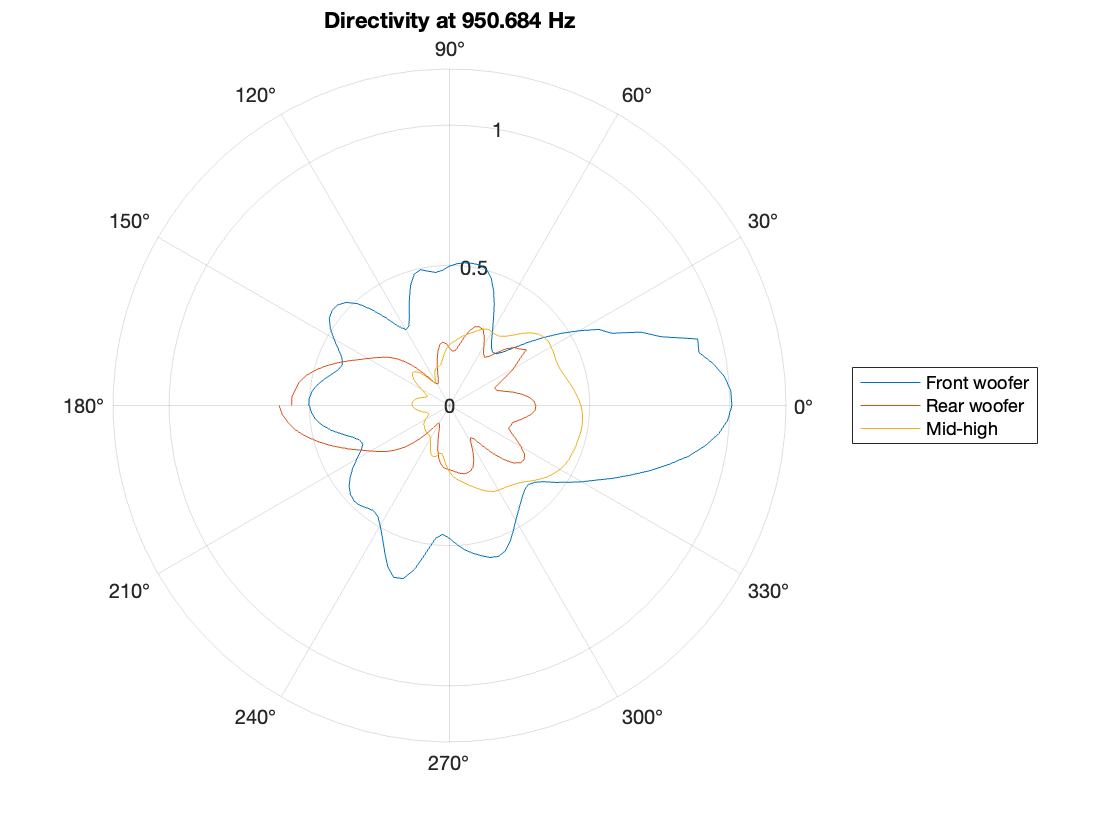
\includegraphics[width = 0.8\textwidth]{figs/initialDirectivity.png}
            \caption{The directivity of each driver in the ACL system at roughly 950Hz.}
            \label{initialDirectivity}
        \end{figure}
        \newpage


        An NTi measurement microphone placed 3.6m away was used to record relative sound pressure levels radiating from the loudspeaker drivers for each frequency at 120 different angles, giving a resolution of three degrees of the $\beta$ axis per measurement.
        The raw results from this measurement were immediately processed; the dataset was large in file size and unwieldy to work with in MATLAB, so the data was reduced in size by taking only every 16th frequency point from the original, unnecessarily large frequency resolution.
        This had no apparent affect on the accuracy or validity of the measurements.

        Upon first inspection of the data, anomalous and invalid pressure-over-frequency data was found at a number of angles.
        Manually cycling through each angle's driver frequency responses, anomalous data was manually averaged out using it's nearest angle neighbors.     

        In hindsight, it would have been more reliable to take a larger number of measurements and find an average over a range of say, a series of twenty measurements, instead of simply averaging an anomalous result with it's angular neighbors.
        However, significant measurement program and signal chain errors were a consistent problem in measurement.
        As so, the number of required measurements to obtain a sufficient level of averaging to smooth out all anomalous results may become impractical.

        Note that the measurements of each driver were taken separately; the cardioid directivity of the LF drivers should be present in their \textit{combined} response.
        Figure \ref{initialDirectivity} does however show a good cardioid directivity pattern for the coaxially mounted KEF Uni-Q.

        The lobing present on the LF driver's directivity response at 1000Hz is to be expected, when inspecting the directivity response below 500Hz the LF drivers behave closer to monopoles.
        However, a clear bias toward the 270 degree measurement angle is also shown, in both the front and rear woofers.
        This may be a cause for concern when designing the rear driver correction filter, however the correction filter may also be used to correct this discrepancy.

        The radiated pressure from the rear driver is shown to be much lower than the front LF driver, this may be due to the fact that the mounting plate for the ELF robot arm was directly over the rear LF driver.
        The coaxial Uni-Q mid high was however mounted over the front driver so this might not be the cause of such a drastic difference, albeit without a protruding metal robot arm in the way.
        Amplifier channels were set to match and the exact same test signal was used for all three drivers, so human experimental set-up error cannot explain the lower rear LF radiation.

    \section{Rear Driver Correction Filter Design}
        \subsection{Spherical Harmonic based Metric and Correction Filter}
            The radiation of the rear driver of the ASL needs to have a particular phase relationship over frequency to radiation of the front driver in order to maintain the rear cancellation required for a cardioid directivity pattern.
            
            Using a metric of cardioid directivity given by Jonathan Hargreaves, previously used and elaborated upon in Vedier's paper, a digital filter was derived to encourage cardioid directivity across the working frequency range of the LF drivers \cite{vedier} \cite{hargreaves2020spherical}.
            When devising this metric, only the zeroth and first spherical harmonics were considered, as a purely cardioid directivity can be described in three dimensions using only these harmonics \cite{vedier}.

            Incorporating higher order spherical harmonics in to a newer, more precise directivity metric may be useful in a further investigation of the non-cardioid directivity behavior of the ACL, but were beyond the scope of this filter design.
            Vedier's work derives a pair of coefficients $a_0$ and $a_1$ from a more general solution to spherical wave propagation, further stating that if these $a$ coefficients are equal, then the radiated pressure waves' directivity must be cardioid.

            Equation \ref{sphericalPressure} shows how spherical harmonic coefficients can be expressed as constituents of pressure in the far field, $p_{ff}$, over spherical angles, where the $R$ term accounts for any residual directivity.

            \begin{equation}
                p_{ff}(\beta,\alpha) = a_0 + a_1 \cos(\beta) + R(\beta,\alpha)
                \label{sphericalPressure}
                \cite{hargreaves}
            \end{equation}

            Using Eq. \ref{a0a1} the coefficients $a_0$ and $a_1$ can be found for the front and rear drivers.
            Both $a_0$ and $a_1$ are derived from terms in a spherical harmonic series, as aforementioned in the literature review.
            This series accounts for axisymmetry in the loudspeaker, and thus $a_0$ and $a_1$, neither of which are dependent on the spherical coordinate angle $\alpha$, can be found as terms in this series.
            This series is given in Eq. \ref{jonSeries}.

            The $b_{m,n}$ in Eq. \ref{jonSeries} and $c_{m,n}$ in Eq. \ref{a0a1} are related by Eq. \ref{related}
            To derive $c_{m,n}$, refer to Eq. \ref{cIntegral}.
            
            \begin{equation}
                p_{ff}(\beta,\alpha,\omega) = \frac{1}{ik} \Sigma_{n=0}^{\infty}i^{-n}b_{0,n}(\omega)\sqrt{\frac{2n+1}{4\pi}}P_n(\cos(\beta))
                \label{jonSeries}
                \cite{hargreaves}
            \end{equation}

            \begin{equation}
                b_{m,n}(\omega) = \frac{c_{m,n}(\omega)}{h_n^{(1)}}
                \label{related}
            \end{equation}

            \begin{equation}
                \begin{split}
                    c_{0,0}(\omega) &= 2\pi^2 \sqrt{\frac{1}{4\pi}}\frac{1}{L}\Sigma_{l=0}^L p(r_{meas},\beta_l,\omega) \times \sin{\beta_l} \\
                    c_{0,1}(\omega) &= 2\pi^2 \sqrt{\frac{3}{4\pi}}\frac{1}{L}\Sigma_{l=0}^L p(r_{meas},\beta_l,\omega) \times \sin{\cos_l} \times \sin{\beta_l}
                    \label{cIntegral}\cite{hargreaves}
                \end{split}
            \end{equation}
            
            \begin{equation}
                \begin{split}
                    a_0(\omega) &= \frac{1}{ikh_0^{(1)}(kr_{meas})} \sqrt{\frac{1}{4\pi}} c_{0,0}(\omega) \\
                    a_1(\omega) &= \frac{1}{ikh_1^{(1)}(kr_{meas})} \sqrt{\frac{3}{4\pi}} c_{0,1}(\omega)
                    \label{a0a1}\cite{hargreaves}
                \end{split}
            \end{equation}

            Equation \ref{a0a1} uses spherical Hankel functions of the first kind, which are a combination of a Hankel function of the first kind and a spherical Bessel functions of the first and second kind \cite{weisstein}.
            The complex exponential component of the given spherical Hankel function characterizes the outwards propagation and decay of a spherical wave; the negative-signed $-e^{ikt}$ component is in contrast to the rest of the positive-signed complex exponentials in the filter generation script.
            Therefore to keep the complex exponential's signs consistent, the complex conjugate of the defined spherical Hankel functions is taken before their use in any calculations.
            The Hankel functions used are defined in Eq.\ref{hankel}, and are derivatives of those given by Wolfram \cite{weisstein}.

            Assuming far-field conditions of measurement allows all directivity terms (spherical harmonics) to be assumed to decay like a monopole.
            This removes any distance dependencies on the overall directivity function, Eq. \ref{sphericalPressure}.

            \begin{equation}
                \begin{split}
                    h_0^1 &= -i  e^{ikr}  \frac{1}{kr} \\
                    h_1^1 &= -e^{ikr}  \frac{kr + i}{kr^2}
                    \label{hankel} \cite{weisstein}
                \end{split}
            \end{equation}

            Conceptually, if the $a_0$ and $a_1$ coefficients are equal, the directivity pattern will be cardioid.
            It should be noted that the response of the $a$ coefficients above 500Hz is mostly irrelevant, as the LF drivers will be filtered out in favour of the Mid-High, which has a favorably cardioid directivity.
            Each driver's $a_0$ and $a_1$ coefficients were derived using the initial frequency and directivity response measurements of the ACL, code used for this is shown in Listing \ref{MATLABsnippet}.

            The mean operators shown on lines 7 and 8 of Listing \ref{MATLABsnippet} are summation-based approximations of the integral over the arc, by way of the trapezium rule \cite{hargreaves}, contained within $c_{m,n}$, shown in Eq. \ref{cIntegral}.
            The resulting $a$ coefficients, while precise, were rough in envelope to the point that a closely matching filter would be unfeasible.
            This can be seen when plotting the immediately derived $a$ coefficients against frequency, shown in Fig.\ref{acoeffsNoSmooth}.
            
            \newpage 

            \begin{lstlisting}[style=Matlab-editor, gobble=16, caption = {MATLAB function used to calculate $a$ coefficients using measured pressure $p$.}, label = {MATLABsnippet}]
                function [a0, a1] = Compute_a_coeff(p, beta, k, r)
                    % Hankel functions (spherical bessel functions with decay):
                    h01 = conj(-1i .* exp(1i .* k .* r) .* (1./(k.*r)));
                    h11 = conj(-exp(1i .* k .* r) .* (((k.*r) + 1i)./((k.*r).^2)));

                    % Computing a_0, a_1 coefficients:
                    a0 = (pi./(2i .* k .* h01)) .* mean(p.*sin(beta),2);
                    a1 = ((3.*pi) ./ -(2.*k.*h11)) .* mean(p.*sin(beta).*cos(beta),2);
                
                end
                
            \end{lstlisting}
            

            Figure \ref{acoeffsNoSmooth} plots both the real and imaginary parts of the calculated $a$ coefficients, and in the real and imaginary parts of $a_0$ and $a_1$ for both drivers, the plot is jagged with high dynamic range between 0-150Hz.
            Whilst any frequencies below 20Hz may be disregarded as inconsequential to a human listener, the 20-150Hz range is within the frequency range where the LF drivers are attempting to give a cardioid directivity.
            Thus, any smoothing applied to this region will have the trade-off of reduced precision and accuracy in the ability of the filter to match the $a$ coefficients in this crucial frequency band.
            
            Finding a good compromise point between the amount post-measurement smoothing and required accuracy in the filter is a point for further study.
            MATLAB's \texttt{smoothdata()} function was used, on it's default setting, to smooth the $a$ coefficients.
            MathWorks describe \texttt{smoothdata()} as a function that: `Returns a moving average of the elements of a vector using a fixed window length that is determined heuristically.' \cite{smoothdata}.

            As the design of the correction filter follows an inverse-FFT methodology, which will be elaborated upon in a further section, only a magnitude response over frequency of the correction filter is needed.
            Therefore, only the magnitude response of the $a$ coefficients was needed to construct the correction filter that makes both $a$ coefficients magnitude equivalent over frequency; this magnitude response can be thought of as an envelope in time without any relevant frequency information, and as such a moving average filter's undesirable frequency characteristics are irrelevant \cite{smith2013digital}.
            Figure \ref{acoeffsSmooth} shows how the moving-average filter has smoothed the $a$ coefficients enough to remove any jagged jumps but keep most of the frequency response's main curves and information.

            The frequency magnitude response of the correction filter was derived by algebraically solving for a hypothetical $\gamma$, the correction filter, across the frequency-domain magnitude of each driver's smoothed $a_0$ and $a_1$ coefficients.
            Equation \ref{gammaAlgebra} shows the magnitude of gamma at each frequency algebraically related to the $a$ coefficients of the front and rear drivers.

            \begin{equation}
                \gamma = \frac{a_{0f} - a_{1f}}{a_{1r} - a_{0r}}
                \label{gammaAlgebra}
            \end{equation}

            Mathematically applying $\gamma$, the derived correction filter, to the rear LF woofer and recalculating the $a_0$ and $a_1$ coefficients for each driver gives a predicted coefficient-over-frequency response shown in Fig.\ref{coeffsPredicted}.

            \begin{figure}[H]
                \centering
                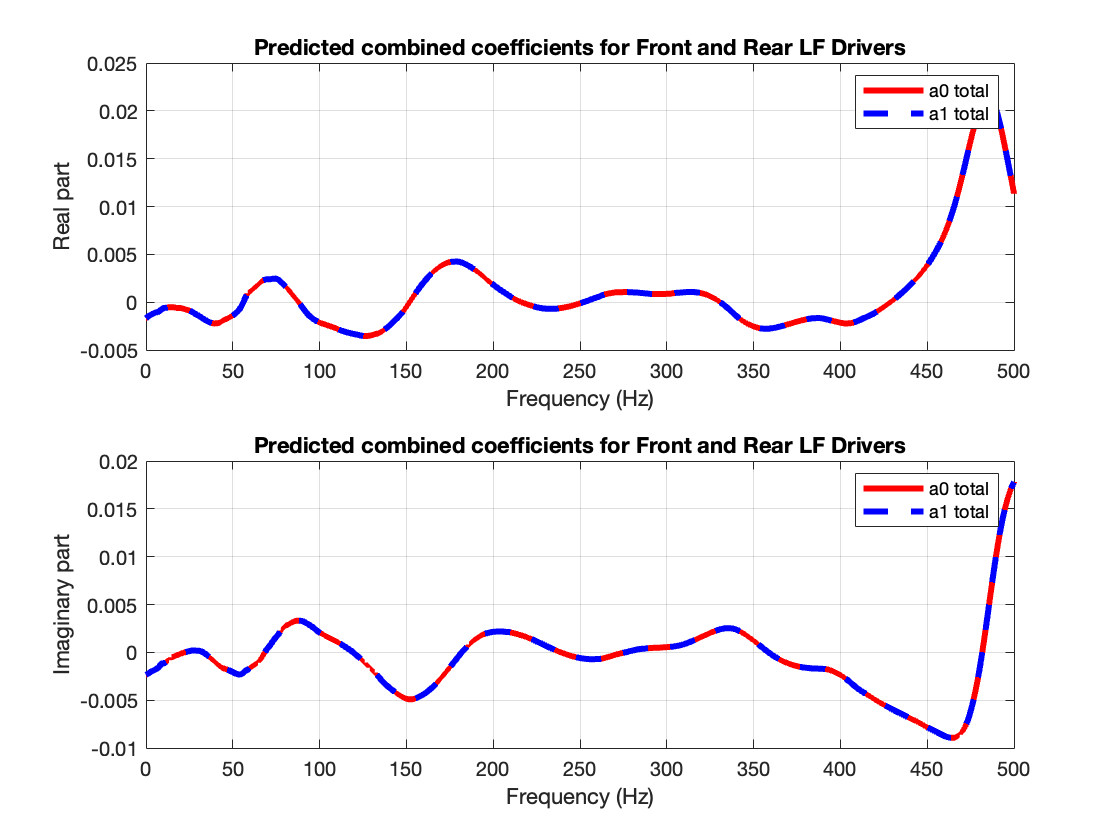
\includegraphics[scale=0.35]{figs/coeffsPredicted.png}%
                \caption{$a_0$ and $a_1$ coefficients remain equal across frequency after $\gamma$ is applied to the measured coefficients.}
                \label{coeffsPredicted}
            \end{figure}

            Looking to Fig. \ref{coeffsPredicted}, a perfect match can be seen, giving validity to the formulation of $\gamma$.
            Both the real and imaginary parts of the new, combined and matching coefficients are much lower in overall amplitude than the measured coefficients seen in Fig. \ref{acoeffsSmooth}.

            Whilst the perfectly matching $a_0$ and $a_1$ coefficients shown in Fig. \ref{coeffsPredicted} are promising, and prove the validity of the algebraic derivation $\gamma$, they are ultimately theoretical.
            Plots of the frequency response, phase response and group delay over frequency of $\gamma$ are given in Fig.\ref{grpDelay}.
            The group delay of a filter determines the time delay that each frequency component of a filtered signal will be subject to \cite{oppenheim1999discrete} \cite{rabiner1975theory}.
            This is an important parameter because, as Olson shows in `Gradient Loudspeakers', the delay between one loudspeaker unit and another in a unidirectional gradient loudspeaker system is a key factor in determining rear cancellation effectiveness.

            \begin{figure}[H]
                \centering
                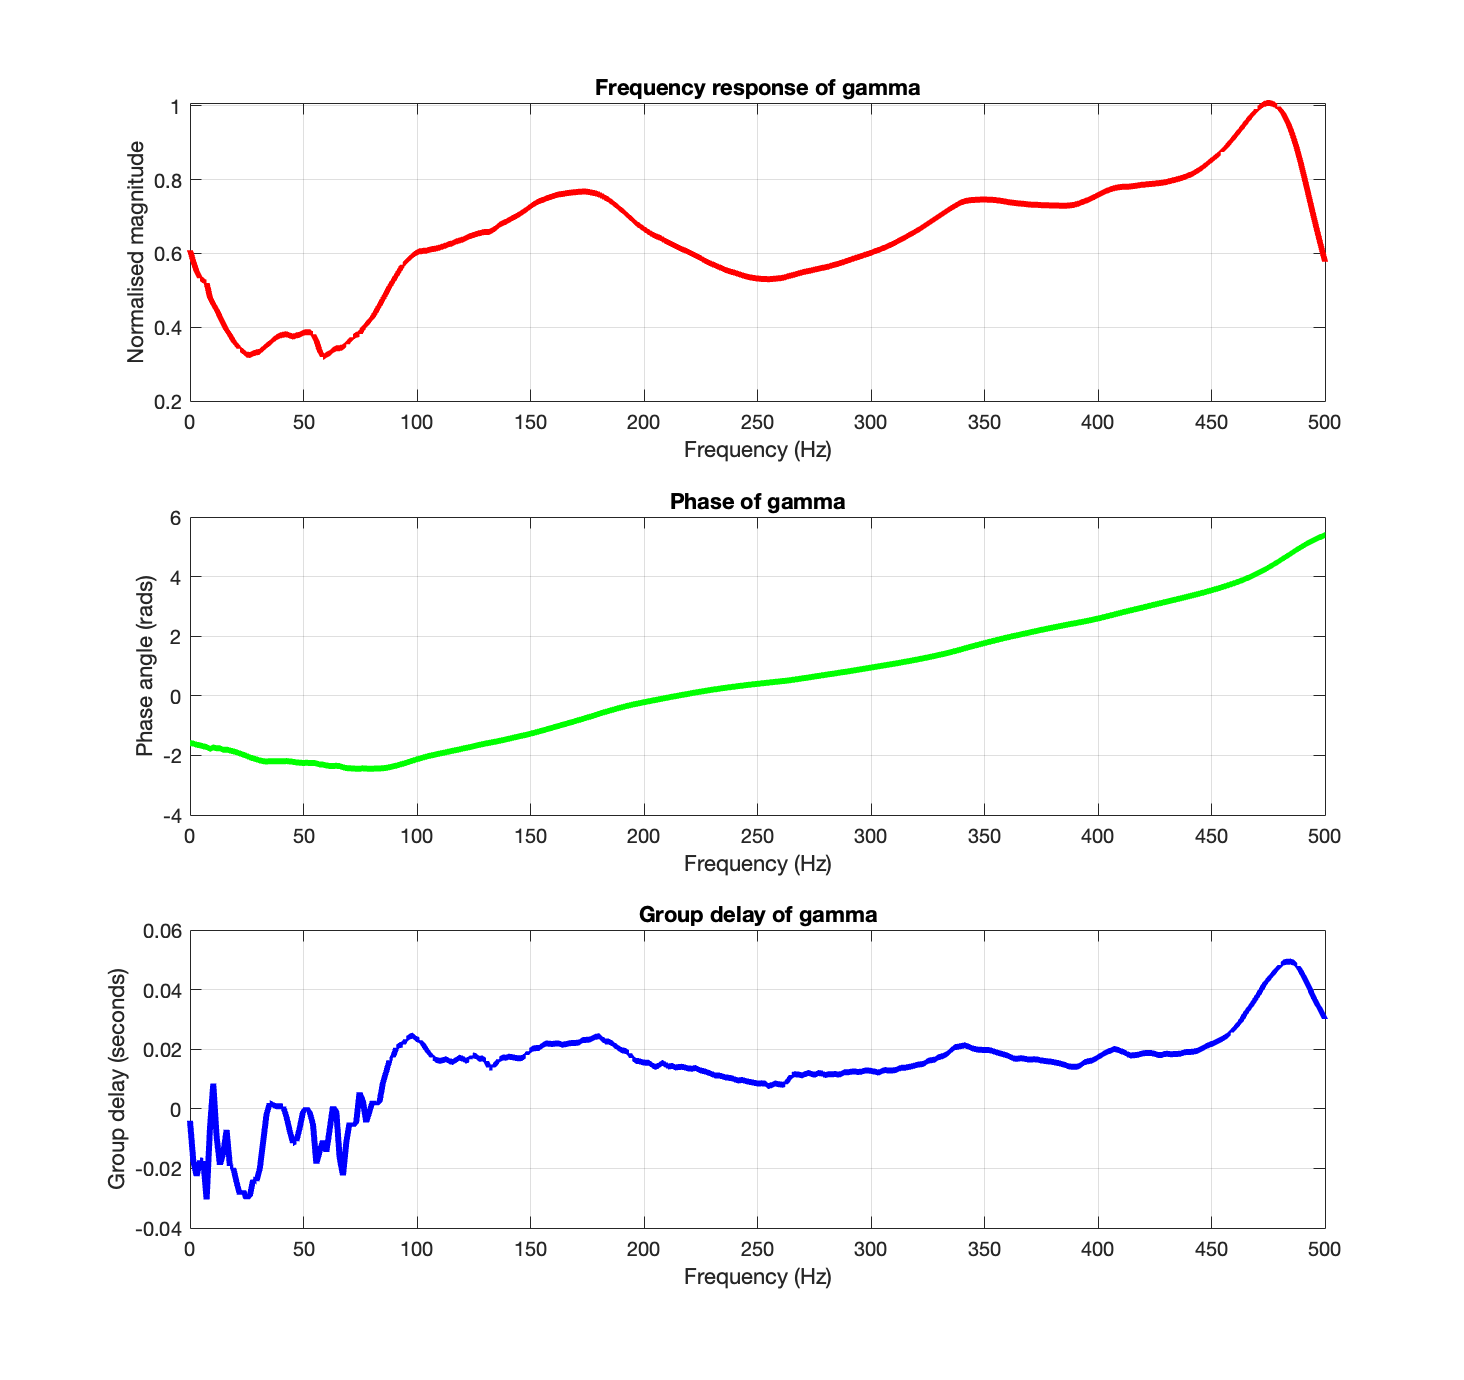
\includegraphics[width = 0.75\linewidth]{figs/grpDelay.png}%
                \caption{Frequency response, phase response and group delay of $\gamma$.}
                \label{grpDelay}
            \end{figure}

            \begin{figure}[H]
                \centering
                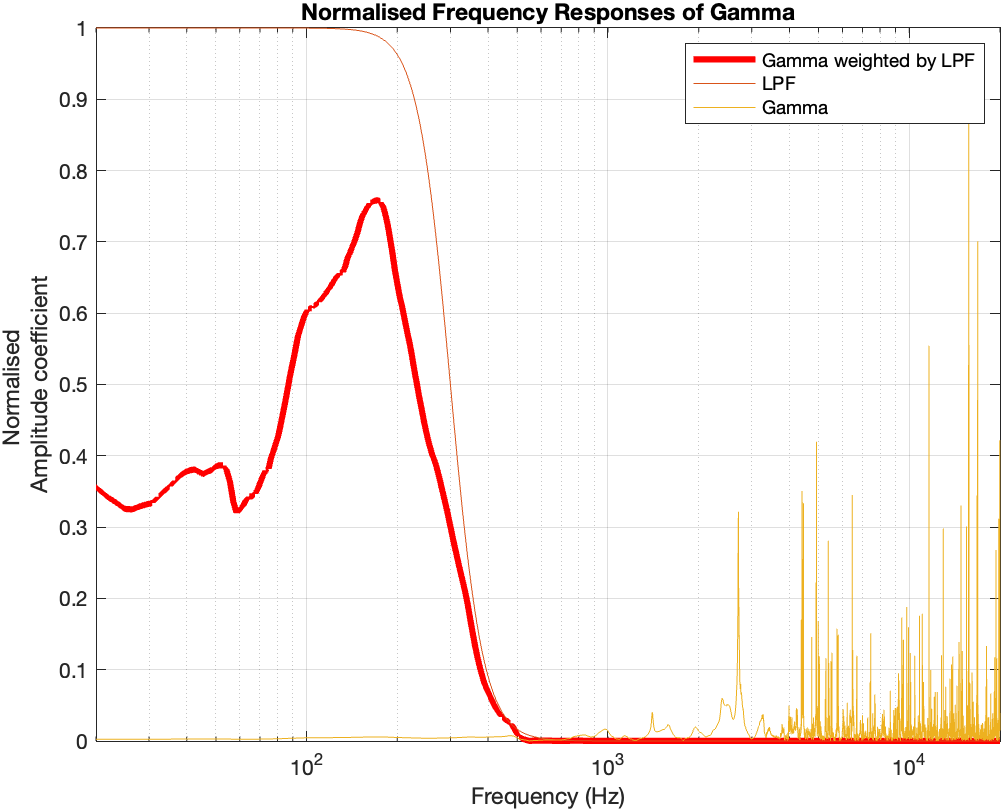
\includegraphics[width = 0.6\linewidth]{figs/gammaCompare.png}%
                \caption{Normalizing $\gamma$ and plotting over the entire frequency range shows the extent of noise above the relevant frequency range.}
                \label{gammaCompare}
            \end{figure}

            Only the rough range of 20-500Hz is relevant to the LF drivers, however, the $a$ coefficients and thus $\gamma$ were calculated across the entire frequency range, up to the Nyquist limit, of the measurement system.
            Upon further inspection of the impact of gamma above 500Hz, unwanted noise and dynamic range is found in the filter, shown by the normalized $\gamma$ in Fig.\ref{gammaCompare}.
            The normalized $\gamma$ has such a degree of noise above it's relevant frequency range that the magnitude in the relevant range is almost unnoticeable.

            In order to eliminate this noise, $\gamma$ was weighted with the frequency response of a 4\^{th} order, 300Hz cut-off, Butterworth low-pass filter (LPF).
            Figure \ref{gammaCompare} shows the affect of the LPF on the normalized $\gamma$, all the unwanted noise is removed and the useful frequency range is unchanged, as it remains in the pass-band of the LPF.
            This presents the next challenge: fitting a real-world implementable filter, including the LPF, to $\gamma$.

            Before progressing to the next section, the amplitudes of the filter frequency response must be discussed.
            Whilst certain plots, such as Fig. \ref{gammaCompare}, normalize the values of the frequency response magnitude coefficients, no actual normalization took place at any time to the frequency response of $\gamma$, before or after filter fitting.
            
            In conclusion, the transfer function of $\gamma$ has now been calculated and is prepared to be fitted to a practical filter.

        \subsection{Correction Filter Implementation}
            A simple, direct and effective way to fit an appropriate filter's magnitude response to $\gamma$ is to use the inverse-FFT method, resulting in a finite-impulse response (FIR) filter.
            The inverse-FFT method of FIR filter design uses an inverse-FFT algorithm to compute the time-domain impulse response of a filter from it's frequency-domain magnitude response \cite{li2019digital}.
            
            As the time-domain impulse response is simply a single finite-length series of scalars, it may be described in the context of FIR filters as a series of $b$ coefficients, where the $a$ coefficients in the in the FIR filter are nonexistent.
            Before taking the inverse-FFT of the $\gamma$ transfer function, it must be weighted (multiplied in the frequency domain) by the LPF.
            Whilst a Butterworth-type frequency response can be manually drawn in MATLAB as an array of weighting coefficients, using MATLAB's \texttt{butter()} function provided easier tweaking of the LPF, as when calling \texttt{butter()}, properties such a filter order can be set.
            MATLAB's \texttt{butter()} generates $a$ and $b$ coefficients of an IIR Butterworth filter, as opposed the FIR desired for $\gamma$.

            Whilst FIR filters are guaranteed, by their finite nature, to decay to zero as stable filters, IIR filters are not, the poles of an IIR filter can, in a pole-zero plot, lay beyond the unit circle, leading to growth instead of decay in the impulse response \cite{litwin2000fir}.
            This can be problematic, and whilst \texttt{butter()}'s design procedure ensures the LPF will be stable the guaranteed stability of FIR filters as opposed to IIR filters was a major factor in choosing to implement $\gamma$ with an FIR filter. 

            \begin{figure}
                \centering
                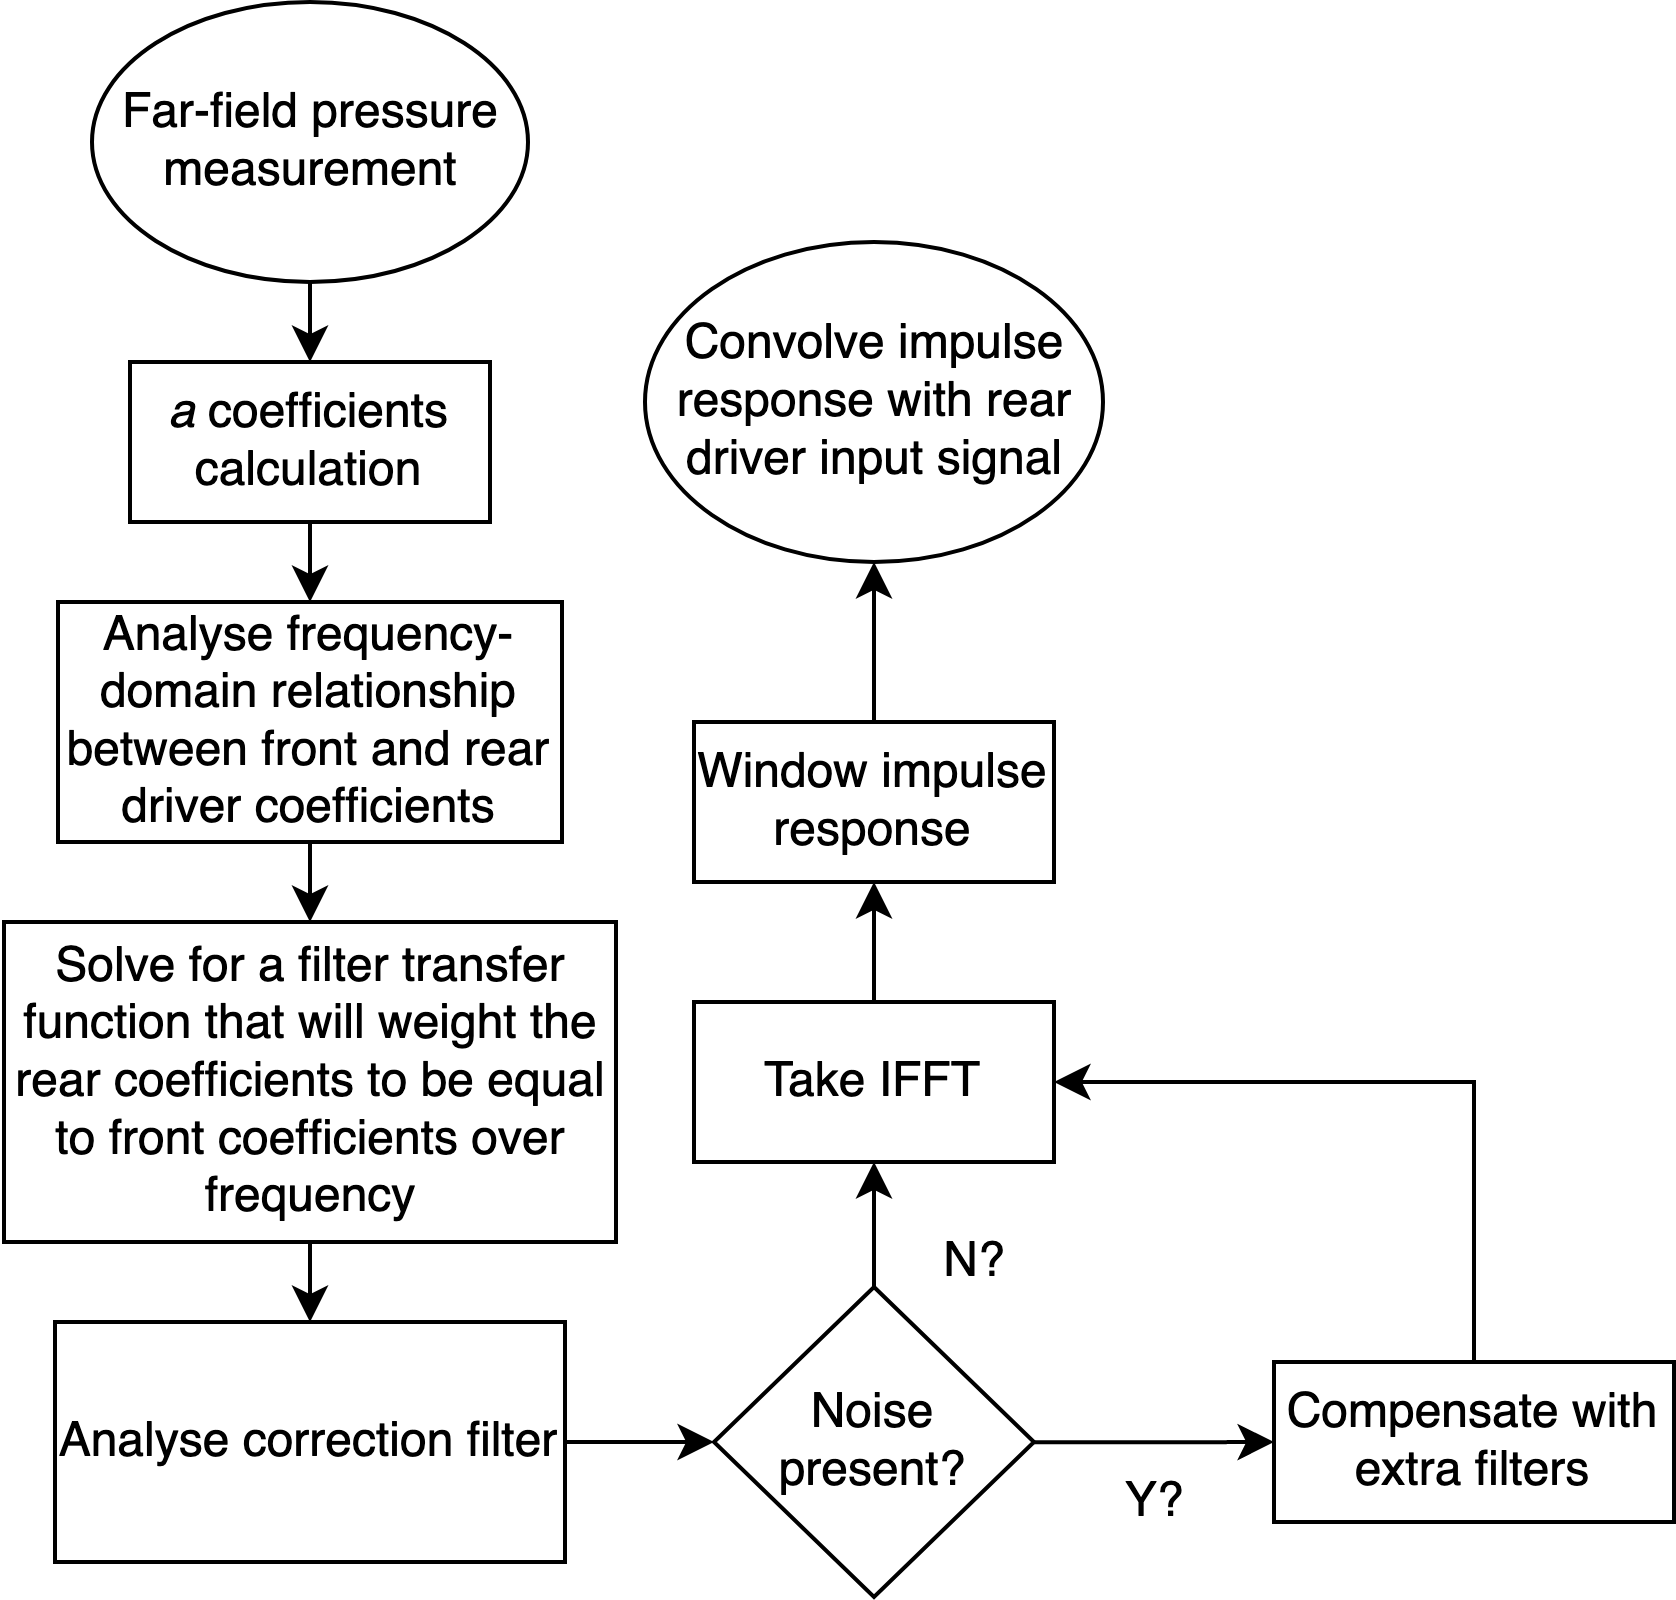
\includegraphics[width = 0.9\linewidth]{figs/filterFlow.png}
                \caption{Flow chart of correction filter design process.}
                \label{filterFlow}
            \end{figure}

            After the Butterworth LPF was generated, MATLAB's in-built \texttt{freqz()} function was used to convert the LPF's $a$ and $b$ filter coefficients into a frequency-domain transfer function.

            From here, the frequency-domain transfer function of the LPF was multiplied with the frequency-domain transfer function of $\gamma$, giving the weighted $\gamma$ frequency response shown in Fig.\ref{gammaCompare}.
            This simple multiplication in the frequency domain should produce no inconsistencies or invalidity of the resultant filter; multiplication in the frequency domain is the same as convolution in the time domain \cite{stanfordConvolution}.
            
            All that was left from this point was to transform the new, weighted $\gamma$ into it's impulse response using an inverse FFT, such that the time-domain effects of the filter can be further investigated.
            The IFFT method of FIR filter design requires some considerations.
            Taking the IFFT of a frequency response in MATLAB will result in an impulse response that is equal in length (in samples) to the frequency response.
            As a precise and complex filter response may require a high resolution in the frequency domain, this may lead to a impractically long impulse response.

            \begin{figure}[H]
                \centering
                \begin{minipage}{.49\textwidth}
                    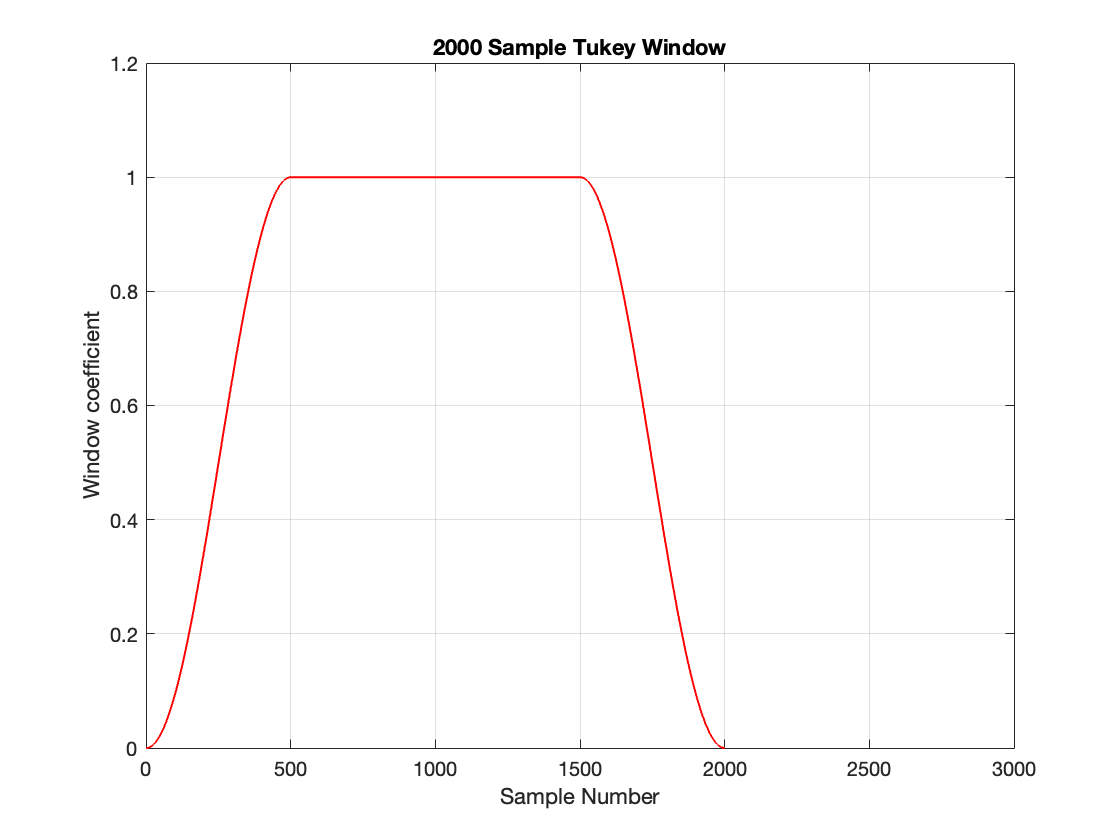
\includegraphics[width=\linewidth]{figs/tukeyWin.png}
                    \caption{Tukey window used to shorten the FIR filter's impulse response.}
                    \label{tukeyWin}
                \end{minipage}
                \begin{minipage}{.49\textwidth}
                    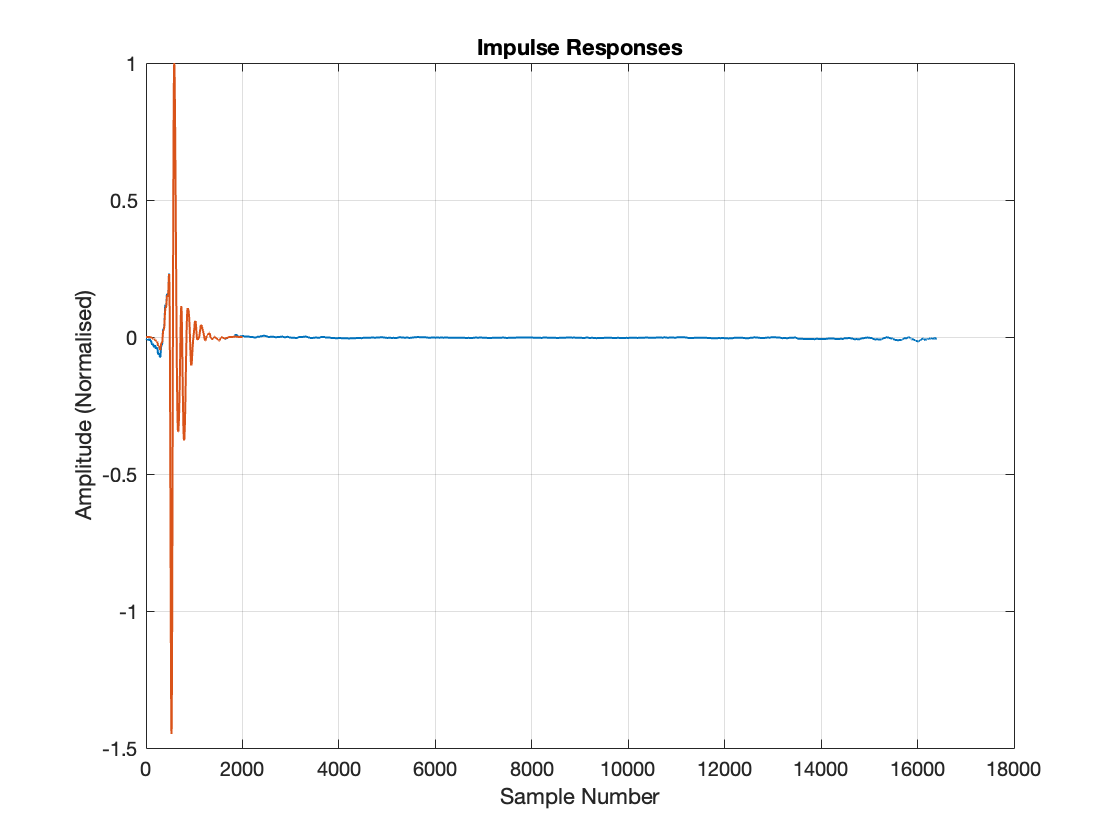
\includegraphics[width=\linewidth]{figs/tukeyImpulse.png}
                    \caption{Windowed and un-windowed impulse responses.}
                    \label{tukeyImpulse}
                \end{minipage}
            \end{figure}

            The generated impulse response, shown in Fig. \ref{tukeyImpulse}, is non-causal and impractically long, with a substantial section wrapped back around $t=0$ to the end of the response, and an increase in amplitude towards the end instead of a continuous trend toward zero.
            This generated audible artifacts and ringing when convolved with any audio signal and played back.

            Thus, the impulse response of the filter was processed to eliminate these problematic characteristics, but preserve it's original frequency and phase characteristics.
            Using MATLAB's \texttt{tukeywin()} function, a window tending towards zero at it's stop bands, was used to keep the useful section of the impulse response and discard the `tail' of the impulse response.

            A brief investigation into the relationship between the width of the window and the error between the windowed impulse response's frequency response and the original impulse response's frequency response was carried out; a window length of 2000 samples was deemed a good compromise between impulse response length and introduced error.

            An FFT of the new, windowed FIR filter impulse response was taken in order to analyze it's frequency and phase performance.
            The phase of the filter, shown in Fig. \ref{tukeyPhase} shows a shift across all frequencies in a similar fashion to the original, longer impulse, almost perfectly matching in the relevant frequency range of the filter.
            This shift however, is not linear and should serve to adjust the phase relationship between the front and rear driver radiation such that sufficient rear cancellation is achieved across the frequency range of the LF drivers.

            Thankfully, a good match in frequency response is also found.
            However, significant smoothing in the sub 100Hz frequency response of the windowed FIR is found, which may lead to a loss in correction precision at these lower frequencies.
            Peaks above the 1000Hz range are also smoothed, but this is beyond the intended range of the filter and is found well past the cut-off of the LPF.
            The impulse response was now ready to be convolved with the rear-driver input signal.
            
            \begin{figure}[H]
                \centering
                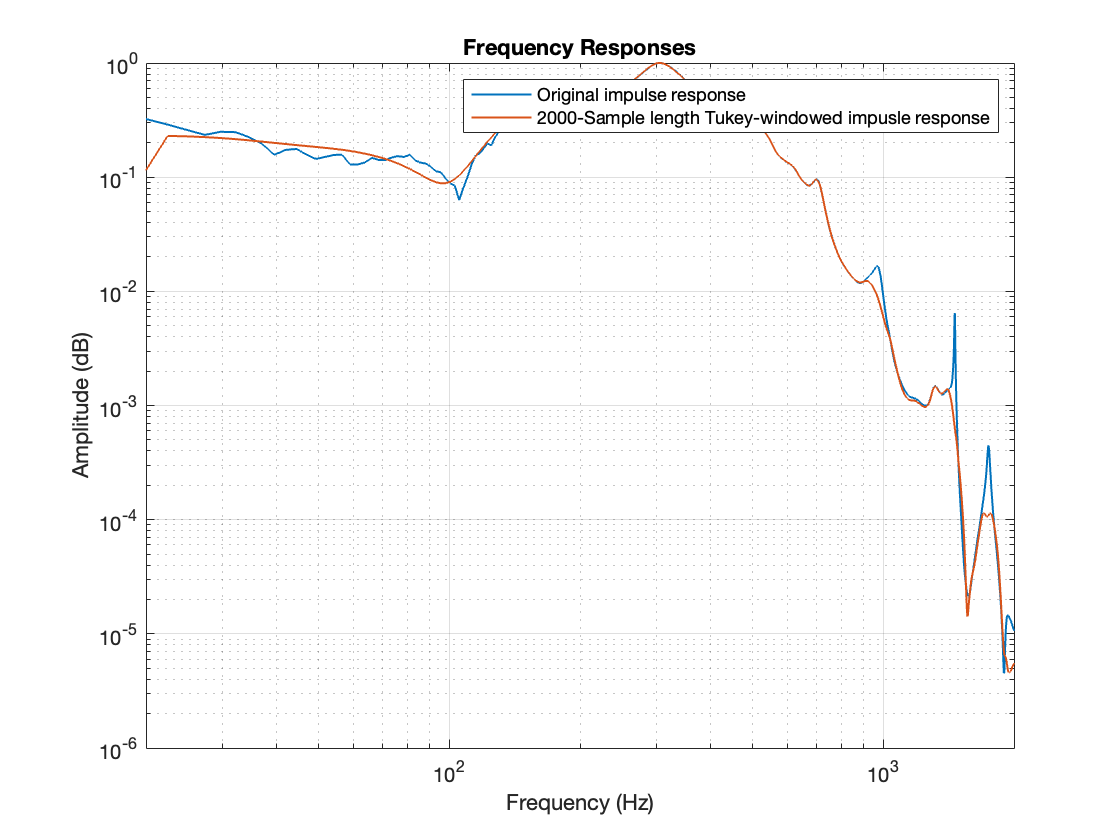
\includegraphics[width=0.7\linewidth]{figs/tukeyFrequency.png}
                \caption{The frequency response discrepancy between the windowed and un-windowed FIR filter.}
                \label{tukeyFrequency}
            \end{figure}

            \begin{figure}[H]
                \centering
                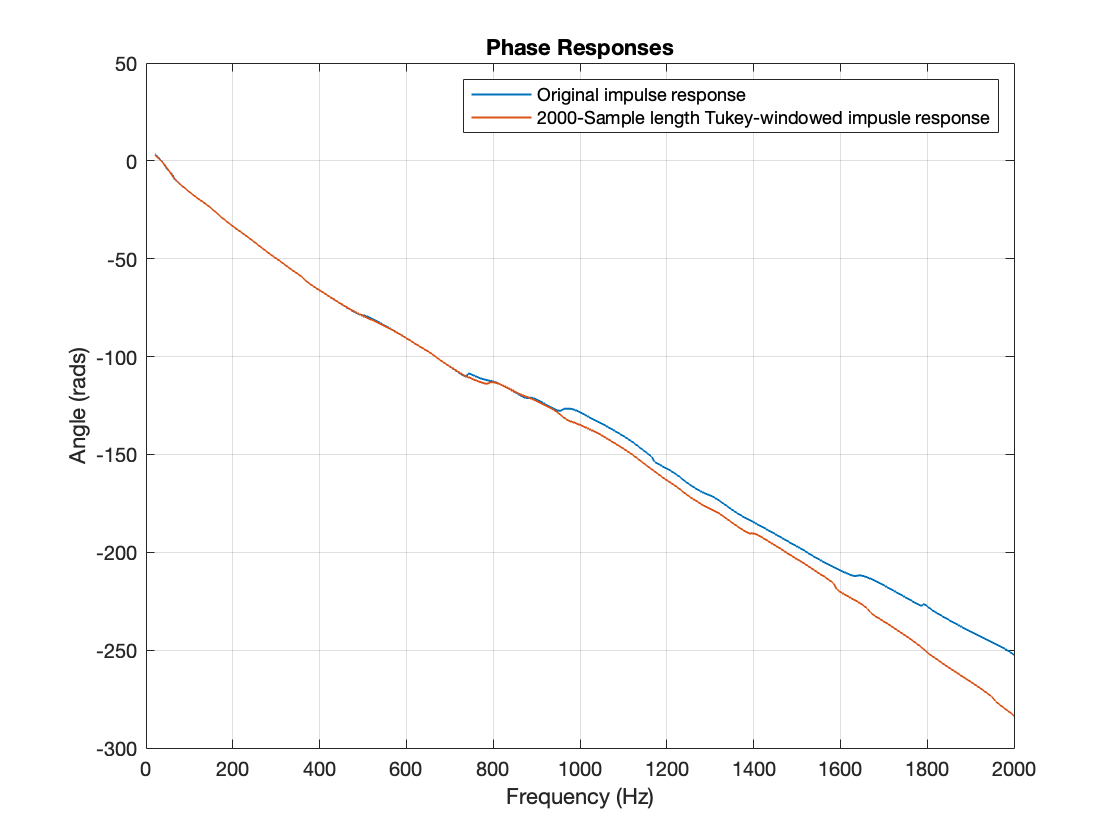
\includegraphics[width=0.7\linewidth]{figs/tukeyPhase.png}
                \caption{The phase response discrepancy between windowed and un-windowed FIR filter.}
                \label{tukeyPhase}
            \end{figure}


            When initially measuring the directivity over frequency of the ACL, swept sine wave excitation signals were fed to all three driver separately.
            However, to analyze the performance of the \textit{combined} LF directivity with the correction filter $\gamma$ applied, the Uni-Q mid-high became irrelevant and as so was not measured a second time.
            The same swept sine test signal was kept, however this time both front and rear LF drivers were fed at the same time, as opposed to the consecutive sweeps of the first test.
            The swept sine fed to the rear driver was convolved with $\gamma$, but the signal fed to the front LF driver remained the same as in the first test.
            
            Apart from the aforementioned differences in test signal play out and included drivers, the testing procedure remained much the same as in Section 4.1.

            It should be noted that at this point in the project, multiple laboratory sessions were required to generate working measurement code and take effective measurements. 
            MATLAB and the general signal chain were delicate, and whilst efforts were made by the Supervisor and Author to automatically re-measure corrupted or problematic measurements, this simply served to complicate the measurement process.
            Thus both this second round of testing, as with the first, had problematic data which needed to be manually identified and smoothed out by averaging a problematic angle's frequency response out with it's neighbors.
            Errors and bad data usually took the form of audio-buffer dropouts, caused either by MATLAB's handling of the system's audio buffer, the ASIO drivers themselves, or some other unknown error.
            These audio dropouts introduced significant noise or error into any angle's frequency response measurement they were present in, mostly to the point where the resulting data from that angle was unusable.
            
            It is possible that some minor playback error went unnoticed, and is even suggested by the notch at roughly 120 degrees on the polar plot of 200Hz combined directivity shown in Fig. \ref{filteredCombinedDirectivity}.
            
            Again, using the code in Listing \ref{MATLABsnippet}, $a$ coefficients were calculated from the directivity functions of the combined loudspeaker.
            Plots of these coefficients are seen in Figs. \ref{filteredaCoeffNoSmooth} and \ref{filteredaCoeffsSmoothed}.

            All in all, the analyzed performance of the windowed FIR correction filter, now the new $\gamma$, was found to be satisfactory.
            However, real-world testing of the filter's impact on combined ACL LF directivity will ultimately determine if the filter, or the theory it is based on, is suitable.

\chapter{Results and Analysis}

    \begin{figure}[H]
        \centering
        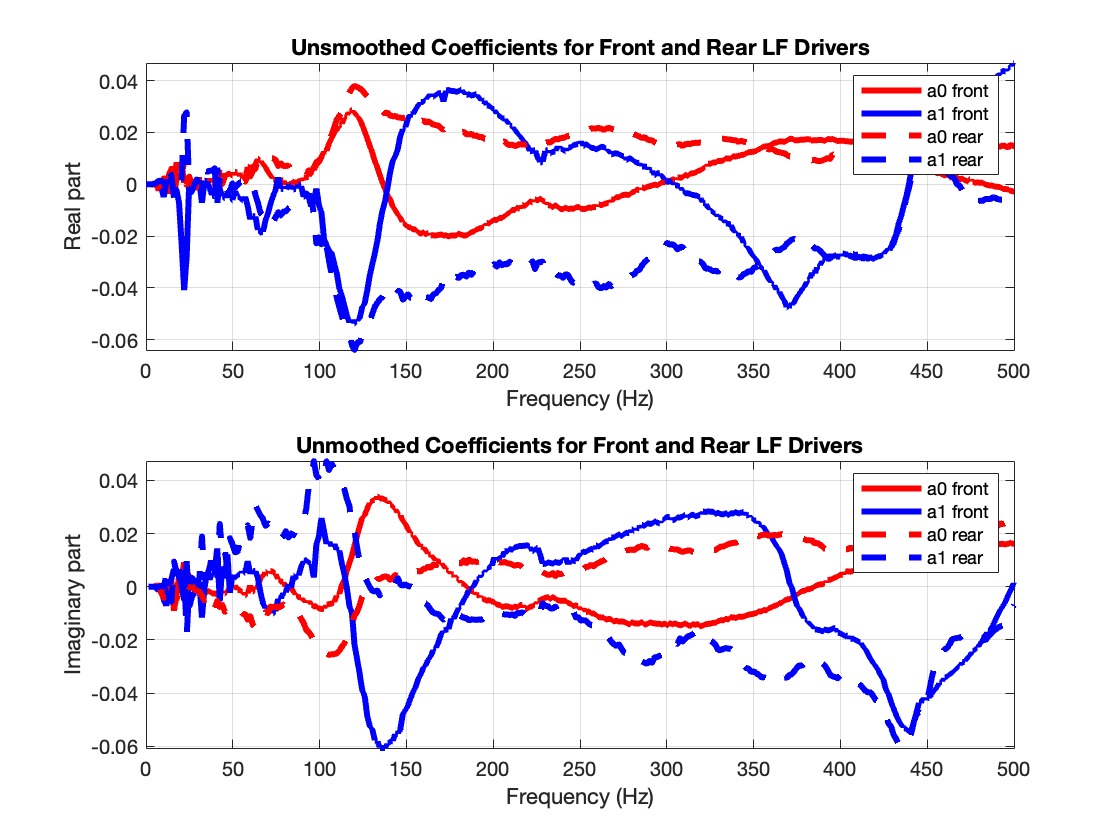
\includegraphics[width = 0.75 \linewidth]{figs/acoeffsNoSmooth.png}%
        \caption{Real and imaginary parts of $a$ coefficients with no smoothing applied.}
        \label{acoeffsNoSmooth}
    \end{figure}

    \begin{figure}[H]
        \centering
        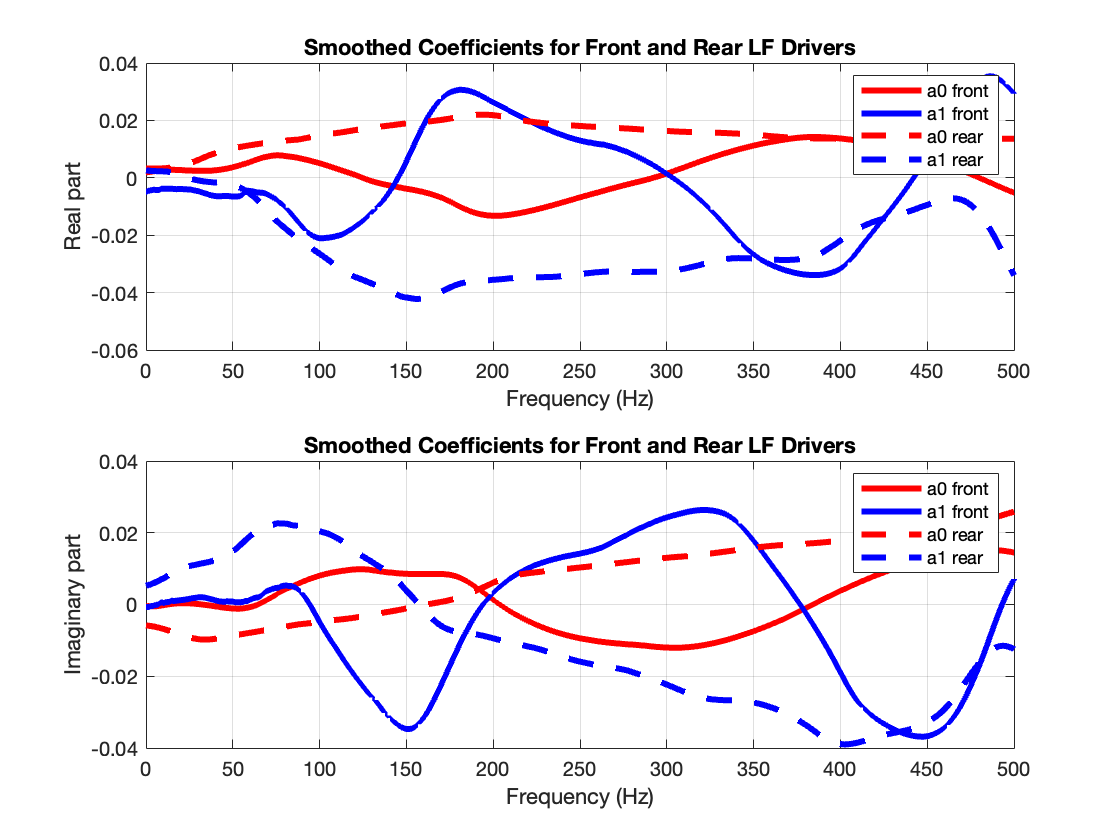
\includegraphics[width = 0.75 \linewidth]{figs/acoeffsSmooth.png}%
        \caption{Real and imaginary parts of $a$ coefficients with smoothing applied.}
        \label{acoeffsSmooth}
    \end{figure}

    \begin{figure}[H]
        \centering
        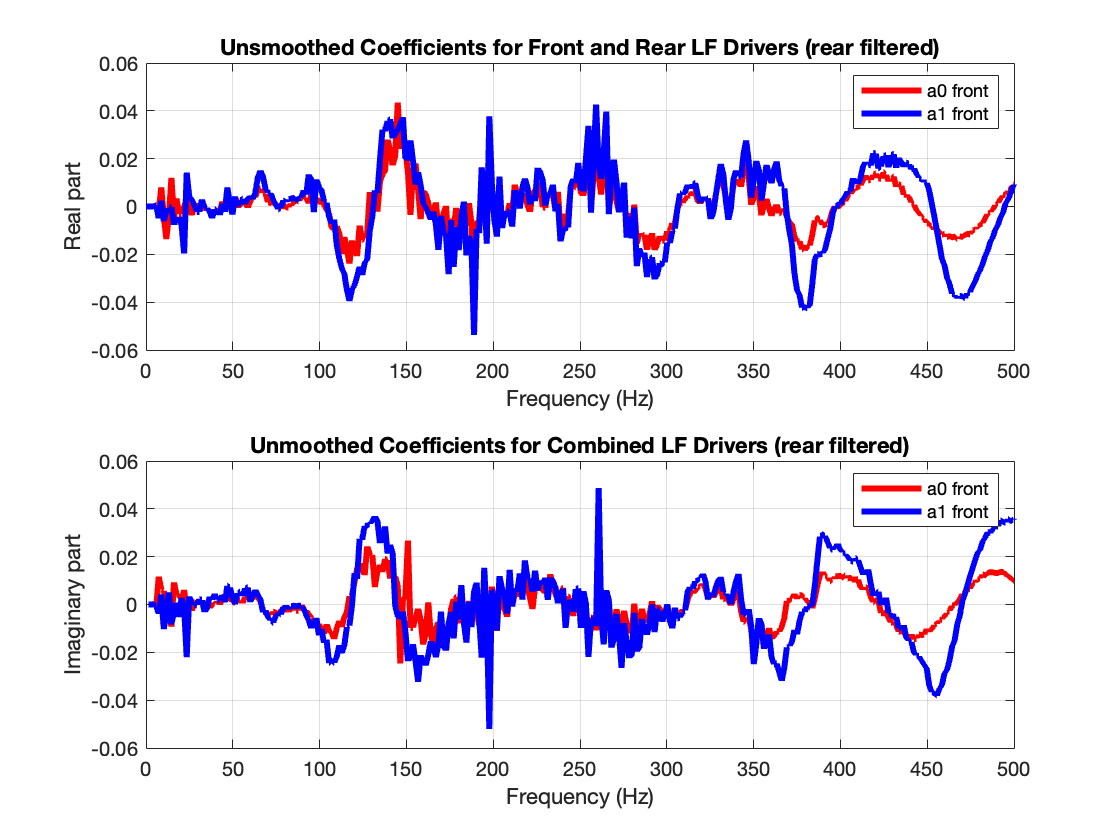
\includegraphics[width = 0.75 \linewidth]{figs/filteredaCoeffNoSmooth.png}
        \caption{Un-smoothed $a$ coefficients of the combined response of the front driver and filtered rear driver.}
        \label{filteredaCoeffNoSmooth}
    \end{figure}

    \begin{figure}[H]
        \centering
        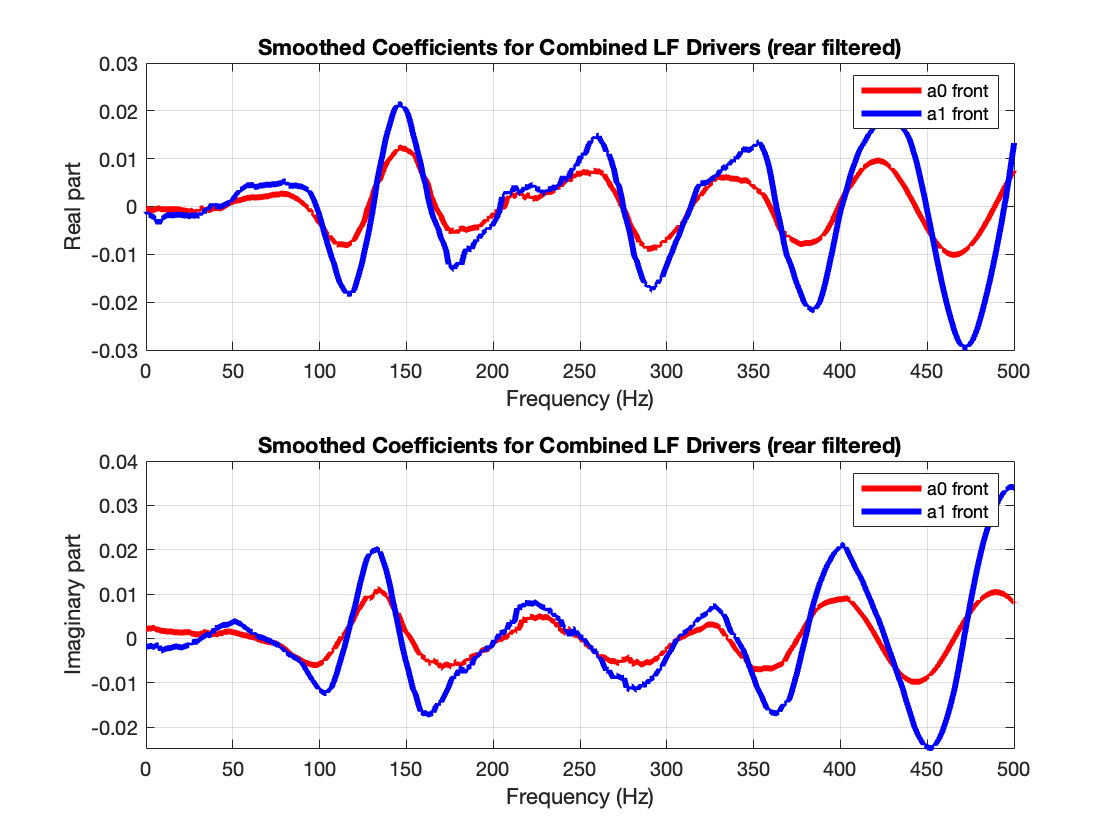
\includegraphics[width = 0.75 \linewidth]{figs/filteredaCoeffsSmoothed.png}
        \caption{Smoothed $a$ coefficients of the combined response of the front driver and filtered rear driver.}
        \label{filteredaCoeffsSmoothed}
    \end{figure}

    \begin{figure}[H]
        \centering
        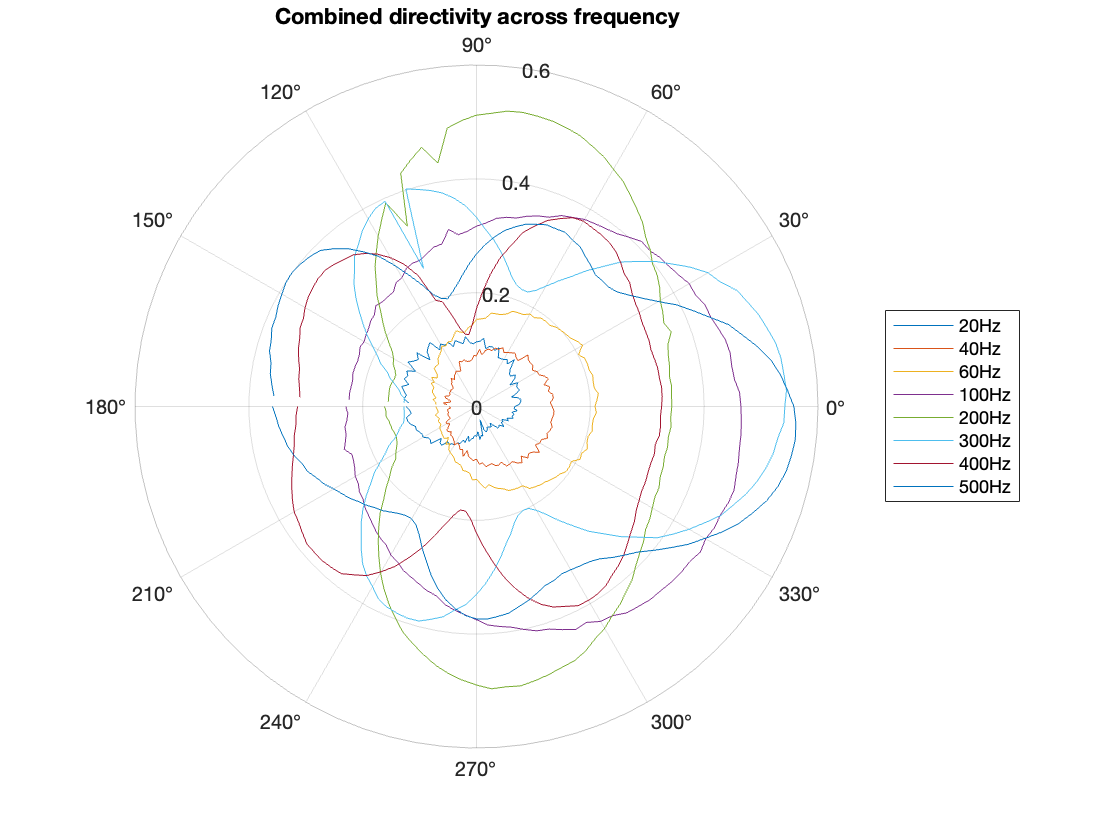
\includegraphics[width=0.8\linewidth]{figs/filteredCombinedDirectivity.png}
        \caption{Filtering the rear and measuring the combined system has shown some change in directivity response.}
        \label{filteredCombinedDirectivity}
    \end{figure}


    Whilst the combined $a$ coefficients shown in Fig. \ref{filteredaCoeffsSmoothed} do not exactly match the mathematical prediction plotted in Fig. \ref{coeffsPredicted}, they do show a good degree of `following' behavior between the coefficients.
    That is, the combined response coefficients follow similar patterns across frequency and deviate much less than the plots in Fig. \ref{acoeffsSmooth}.
    The dramatic lowering in absolute value of coefficients shown by the predictions in Fig. \ref{coeffsPredicted} did not manifest; the absolute values of the $a$ coefficients pre and post filtering remain in similar magnitude bands.
    However, it cannot be expected that real-world performance will perfectly mirror a simple algebraic solution that makes a great deal of assumptions.

    Figure \ref{filteredCombinedDirectivity} depicts the combined directivity response of the LF drivers over a range of frequencies.
    It is clear to see that at particular frequencies (200Hz, 300Hz), a fairly cardioid directivity pattern is reached with clear rejection at 180 degrees, the rear of the ACL.
    Whilst other frequencies do not have as `cardioid' a polar pattern, every plot that crosses the 0.4-magnitude line of the polar, crosses it only in the on-axis (0 degrees) region.
    Thus, some degree of rear rejection across all frequencies, at least compared to the on-axis radiation, is achieved.

    Comparing the directivity at 200Hz to Vedier's polar plot in Fig. \ref{vedierPolar} an almost half-way point is reached, by the combined directivity, between the polar patterns of the presented analytical and FEM solutions.
    Remembering that Vedier's simulations did not account for the coaxial mounting of the Uni-Q, some discrepancy is to be expected.
    However, it's hard to explain why exactly the discrepancy took the form it did.

    The polar plot of Olson's first-order unidirectional gradient loudspeaker, seen in Fig. \ref{olsonFirstOrderDirectivity}, is much more optimistic and ideally cardioid, matching the polar pattern typically given by a cardioid microphone.
    As aforementioned in the Literature Review, Olson's gradient loudspeakers are the sums of perfect monopoles, which the LF drivers, or any driver for that matter, are not; the imperfect result obtained is to be expected.

    Non-cardioid features of the polar plots in Fig. \ref{filteredCombinedDirectivity} may be explained by the residual, higher spherical harmonic order, pressure $R$, found in in Eq. \ref{sphericalPressure}.
    To investigate the contributions of $R$ using Eq. \ref{sphericalPressure}, a far-field assumption of monopole-like decay must be applied to the higher order spherical harmonics, as was applied to the lower-order spherical harmonics \cite{hargreaves}.
    This may prove difficult or unwieldy, so the residual will be calculated in terms of the measured radius of the pressure radiation.

    \begin{equation}
        R_{meas}(\beta,\alpha,\omega) = p_{meas}(r_{meas},\beta,\alpha,\omega) - ikh_0^{(1)}(kr{meas}) \times a_0(\omega) + kh_1^{(1)}(kr{meas}) \times a_1(\omega)\cite{hargreaves}
        \label{residualEquation}
    \end{equation}

    Equation \ref{residualEquation} shows that by multiplying each $a$ coefficient by the Hankel function used to form it, the residual pressure as a result of higher-order spherical harmonics $R$ can be calculated.
    This is simply a re-arranging of Eq. \ref{sphericalPressure} accounting for the mapping of the Hankel functions as seen in Listing \ref{MATLABsnippet}.

    \begin{figure}[H]
        \centering
        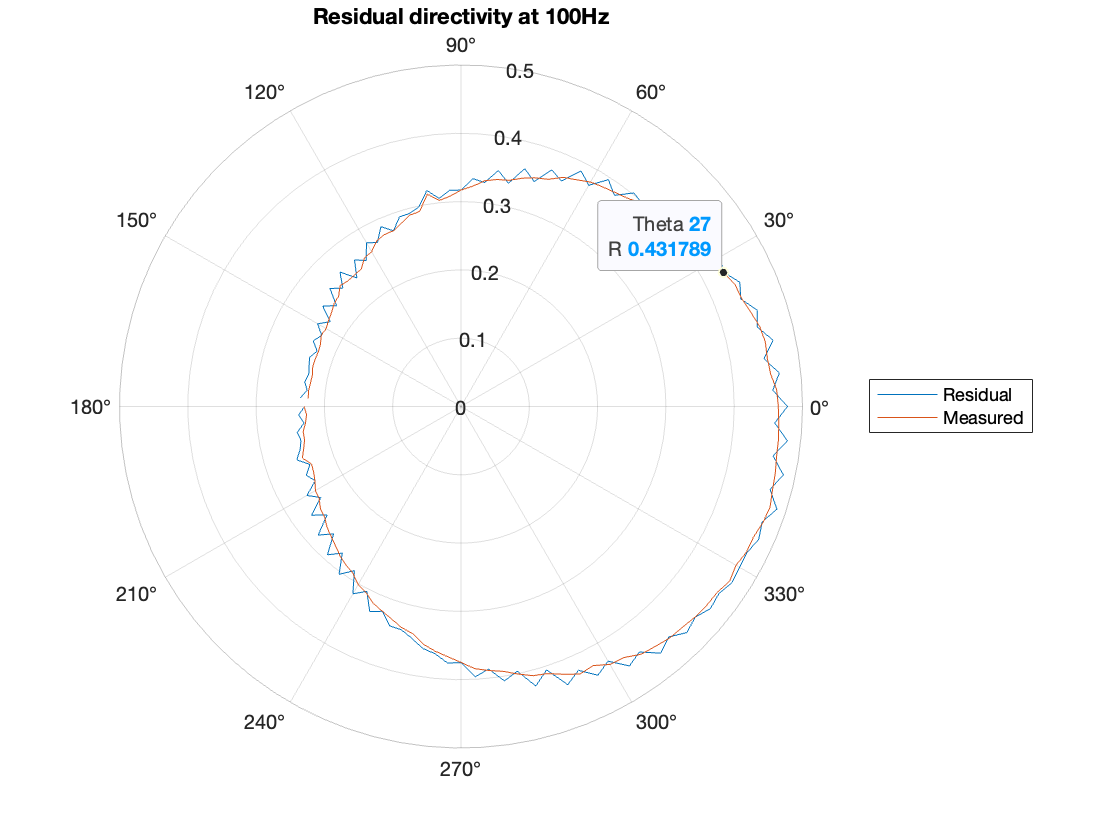
\includegraphics[width=0.8\linewidth]{figs/residual100.png}
        \caption{Residual Directivity at 100Hz}
        \label{residual100}
    \end{figure}

    \begin{figure}[H]
        \centering
        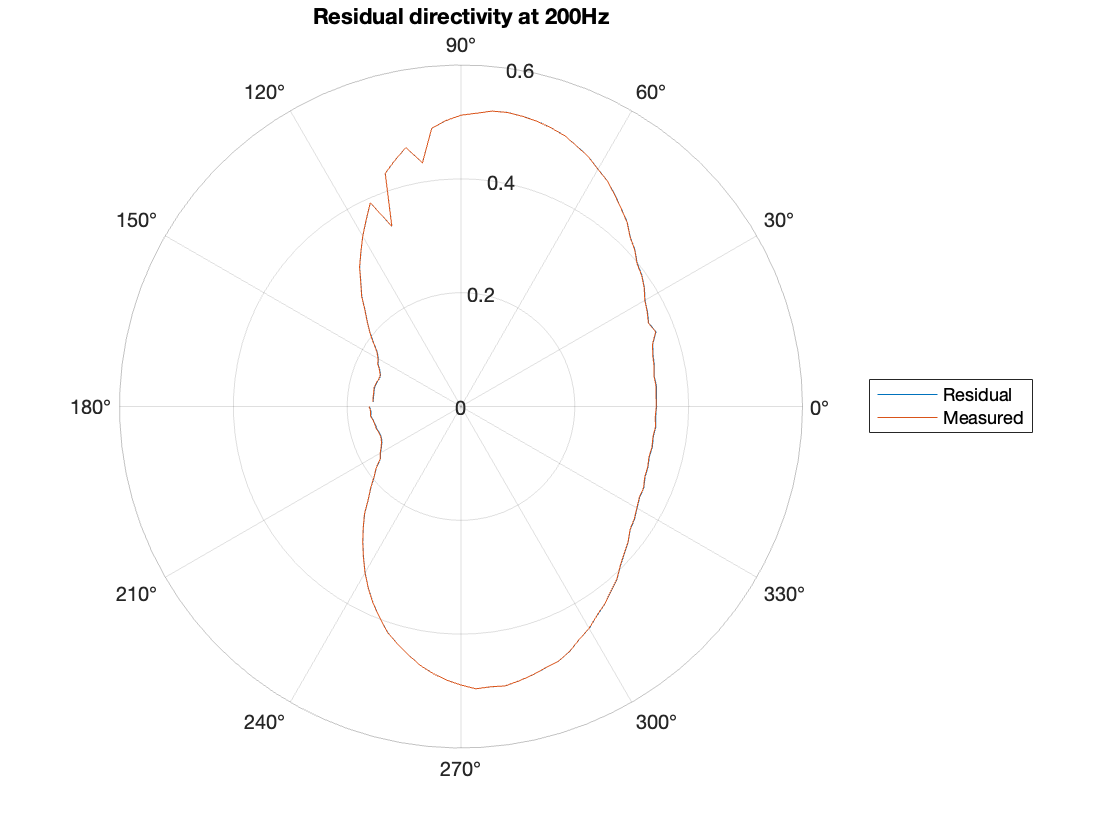
\includegraphics[width=0.8\linewidth]{figs/residual200.png}
        \caption{Residual Directivity at 200Hz}
        \label{residual200}
    \end{figure}

    The residual pressure information, shown by Figs. \ref{residual100} and \ref{residual200} does not particularly deviate from the total measured pressure in the far-field.
    This may be due to a minimal contribution of higher order spherical harmonics, which is unlikely, or an error in calculation of the residual $R$.
    It was decided that this is an inappropriate way to formulate the residual, and that taking it as a function of frequency, like the $a$ coefficients, was more appropriate.

    \begin{figure}[H]
        \centering
        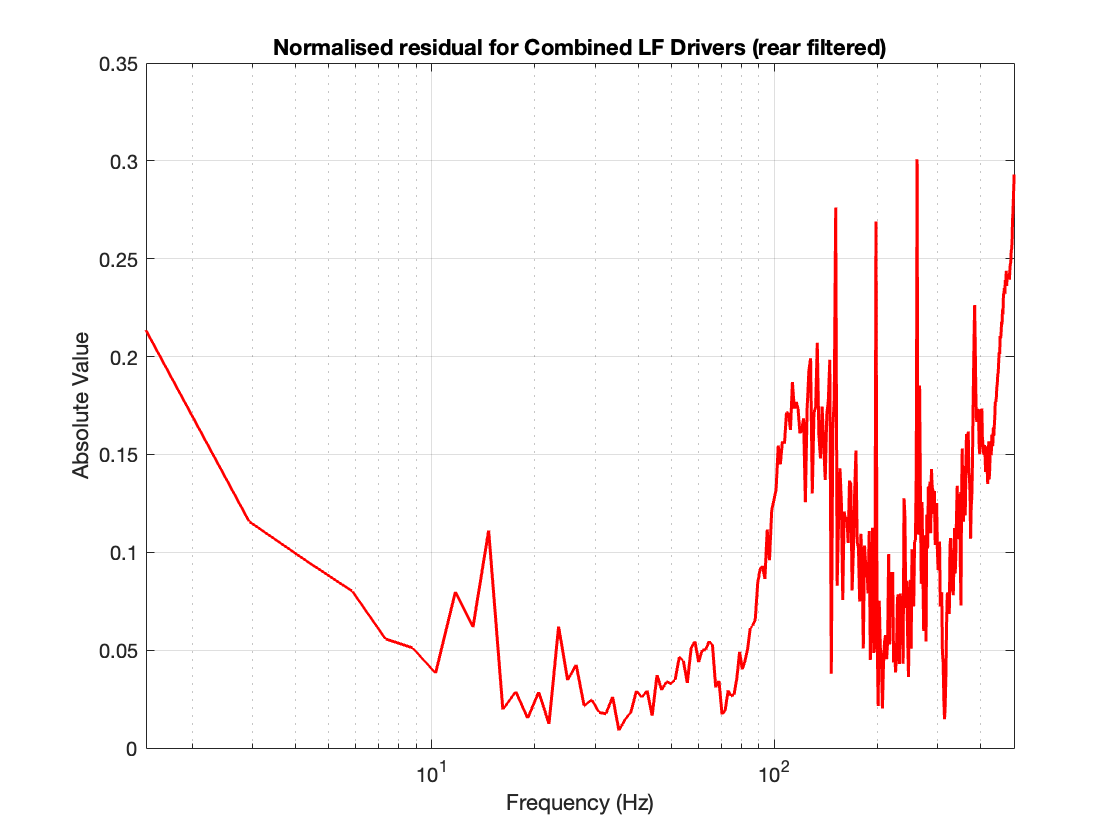
\includegraphics[width=0.8\linewidth]{figs/residualOverf.png}
        \caption{Combined residual `coefficient' over frequency calculated using Eq. \ref{residualEquation}.}
        \label{residualOverf}
    \end{figure}

    The increase in residual value $R$ as frequency increases shown by Fig. \ref{residualOverf} is to be expected, this suggests this residual directivity function over frequency may be used as the basis for further directivity correction filtering.

    Plotting the combined directivity at the frequency corresponding to a quarter wavelength, 139Hz, does not correlate well to the suggested distance-introduced phase shift rear cancellation that should give a cardioid response, as suggested by Olson and others.
    Once again, this may be due to non-monopole directivity from each LF driver pushing this effect to another frequency, or damping it entirely.
    Notches between 120 and 90 degrees are again visible, probably due to sine sweep playback dropouts during testing.

    In conclusion, whilst analysis of the residual directivity as a result of higher order spherical harmonic pressure was in polar plots was unfruitful, some expected behavior is shown by plotting the residual as a function of frequency, averaged over all angles.
    The correction filter was shown to encourage matching of the $a$ coefficients over the frequency range of the LF drivers. 

\chapter{Discussion and Conclusions}
    Analyzing contemporary sound field control literature shows axisymmetric and cardioid designs are both beneficial to sound field control applications.
    The ACL seems a particularly good candidate for Chang and Jacobsen's circular double-layer array of loudspeakers, a technique that seeks to not only create dark and bright acoustic zones, but also control the sound field within the bright zone.

    Comparing the measured $a$ coefficients pre and post filtering shows the filter made some progress toward achieving a more cardioid directivity pattern in the low frequency range, or at least that the filter made progress towards matching the combined drivers' $a$ coefficients over their frequency range.
    When attempting to analyze the directivity of higher-order spherical harmonics, a plot of residual higher-order spherical harmonics in terms of Eq. \ref{sphericalPressure} was found, and showed an expected trend of greater residual pressure at higher frequencies.

    The literature also shows that characterizing loudspeaker directivity in terms of spherical harmonics is a common contemporary research technique.
    However, the simplified coefficient based model was not found elsewhere in the literature.
    This is not to say that no-one has attempted this method, just that it is not so commonplace to be easily found.
    This leaves the $a$ coefficient based far field pressure equation (Eq. \ref{sphericalPressure}) open to deeper investigation and testing.

    The second laboratory session, documented in the attached logbook, failed to return any results due to equipment problems.
    The first two days of the third laboratory were unfortunately similar.
    This limited the scope of this project and meant that any real-world qualitative performance of the ACL were not documented.
    Repeating the quantitative measurements undertaken in this test would serve to improve the accuracy of measured results; statistical analysis of results may also suggest sources of error in the testing methodology.

    The directivity measurement method used in this project, that is, mounting the loudspeaker on a rotating robot arm and taking sine sweep transfer function measurements every three degrees over a full 360 degree rotation, was shown to be effective, even if the signal chain experienced some practical issues.
    
    In conclusion, whilst the scope of this project was ultimately limited, a successful demonstration of the feasibility of implementing a spherical harmonic based directivity correction filter to the ACL was achieved.
    The reaction of the derived combined $a$ coefficients when subjected to filtering was demonstrated, having strong correlation to expected real-world directivity over frequency behavior when analyzing the residual, and opens the door for further work in this domain.
    Suggestions for further work are discussed in the next chapter.

\chapter{Further Work}
    This project left a number of unanswered questions and points for further investigation.

    First, facets of the loudspeaker's construction may be investigated.
    The suitability of each KEF driver for this particular ACL should be investigated and documented, such that any future work may be better informed as to their suitability.
    Investigations of the length and overall volume of the coupled chamber and thus the ACL as a whole would be beneficial; the assembled unit is relatively large and unwieldy, albeit not too large when compared to contemporary PA loudspeakers which often need more than one person at a time to transport.
    
    Experimenting with a spherical enclosure as suggested in `Direct Radiator Loudspeaker Enclosures' may give noteworthy results, but it should be noted that spherical loudspeaker constructions are not without their issues \cite{olson1969direct}.
    Integrating crossover filtering, compensation filtering, amplification and a better performing rear-driver correction filter into the assembly of the prototype ACL would bring it into the domain of a practical, modern active PA speaker.
    
    KEF's Ci250RRM-THX LF driver cavity resonance issues and their compensation through an open-back Uni-Q driver provide inspiration to investigate if similar cavity resonances are present at the front LF driver of the ACL.
    If so, KEF's method of opening the back of the Uni-Q may be tried and compared to newer, experimental methods of cavity resonance compensation.
    Remaining on the topic of loudspeaker construction, an investigation in to whether the coupled acoustic chamber of the ACL performs as suggested in Jordan Cheer's `Robustness and Efficiency' \cite{cheer2015robustness}.
    
    Both Quantitative and Qualitative analysis of the ACL's performance as part of a sound field control installation should serve to give a better frame of purpose to the ACL project.
    The scope of ACL performance measurements may also be expanded and informed by measurements of each individual driver with a laser doppler vibrometer, this may help to better characterize the acoustic relationship between each driver and thus the correction filter.
    
    The effect of $a$ coefficient smoothing and a study of convergence between the order of smoothing and correction filter performance may prove insightful.
    However, the precision of the filter is ultimately limited by computation power and filter feasibility.

    As aforementioned, the residual directivity function over frequency, given in Fig. \ref{residualOverf} may serve as a useful starting point for further research into correcting the non monopole and dipole directivity of the combined LF driver directivity.

    Overall, the scope for further work on this project remains open and large, and the author (that's me!) hopes the supervisor takes the prototype ACL further towards a working, useful state.

\bibliographystyle{IEEEtran}
\bibliography{theBib.bib}

\end{document}


